\renewcommand{\figurename}{Diagram}
\subsection{Merge Tracking}

Subversion supports per-directory and per-file merge tracking. The implementation of per-branch merges built on top of per-directory merges. Git tracks per-branch merges only. Hence Translator is able to translate branch-level merges only. In this section we consider common merge scenarios and describe the behavior of Translator for every of them.

\subsubsection{Merge History Basics}

Subversion keeps the history of merges performed on certain branch. It is represented as svn:mergeinfo property set on branch root directory. When Git user performs merge from branch2 to branch1, all commits of branch2 becomes the history of branch1. From Subversion perspective that means that branch1 got branch2 as merge history, i.e. svn:mergeinfo property should include revisions mapped to merged commits. This idea illustrated on diagrams \ref{simple_merge_git_to_svn} and \ref{simple_merge_branch_no_parent_git_to_svn}.

\begin{center}
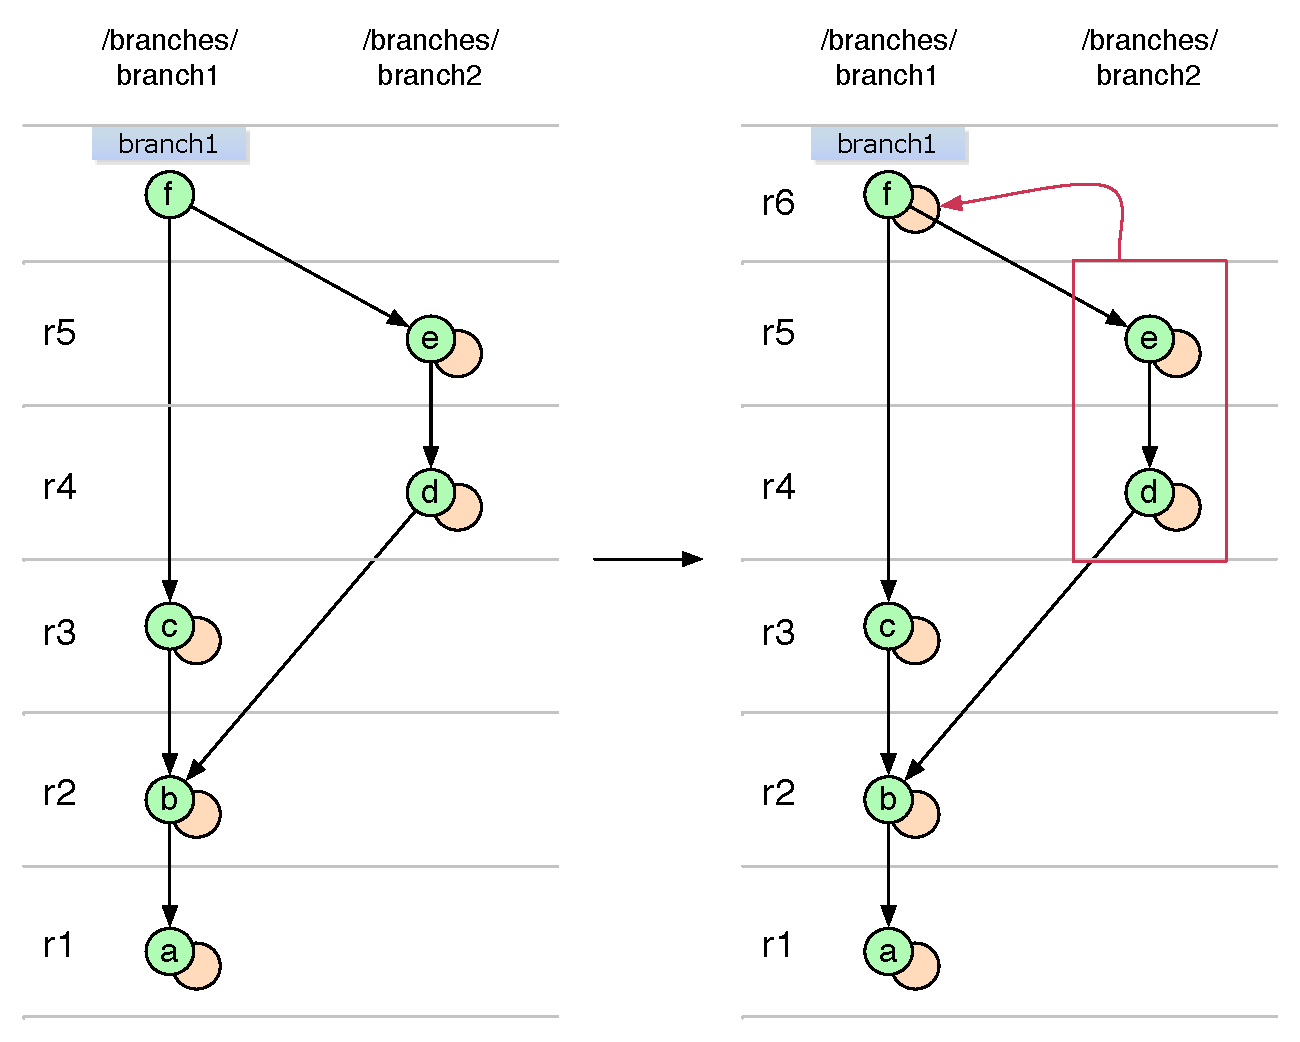
\includegraphics[width=\textwidth]{img/diagrams/simple_merge_git_to_svn.pdf}%
\captionof{figure}{Git merge commit being translated to the change of svn:mergeinfo property.}
\label{simple_merge_git_to_svn}%
\end{center}

The difference between these scenarios is that merged branch2 branch may have common commits with branch1 or no common commits at all.

\begin{center}
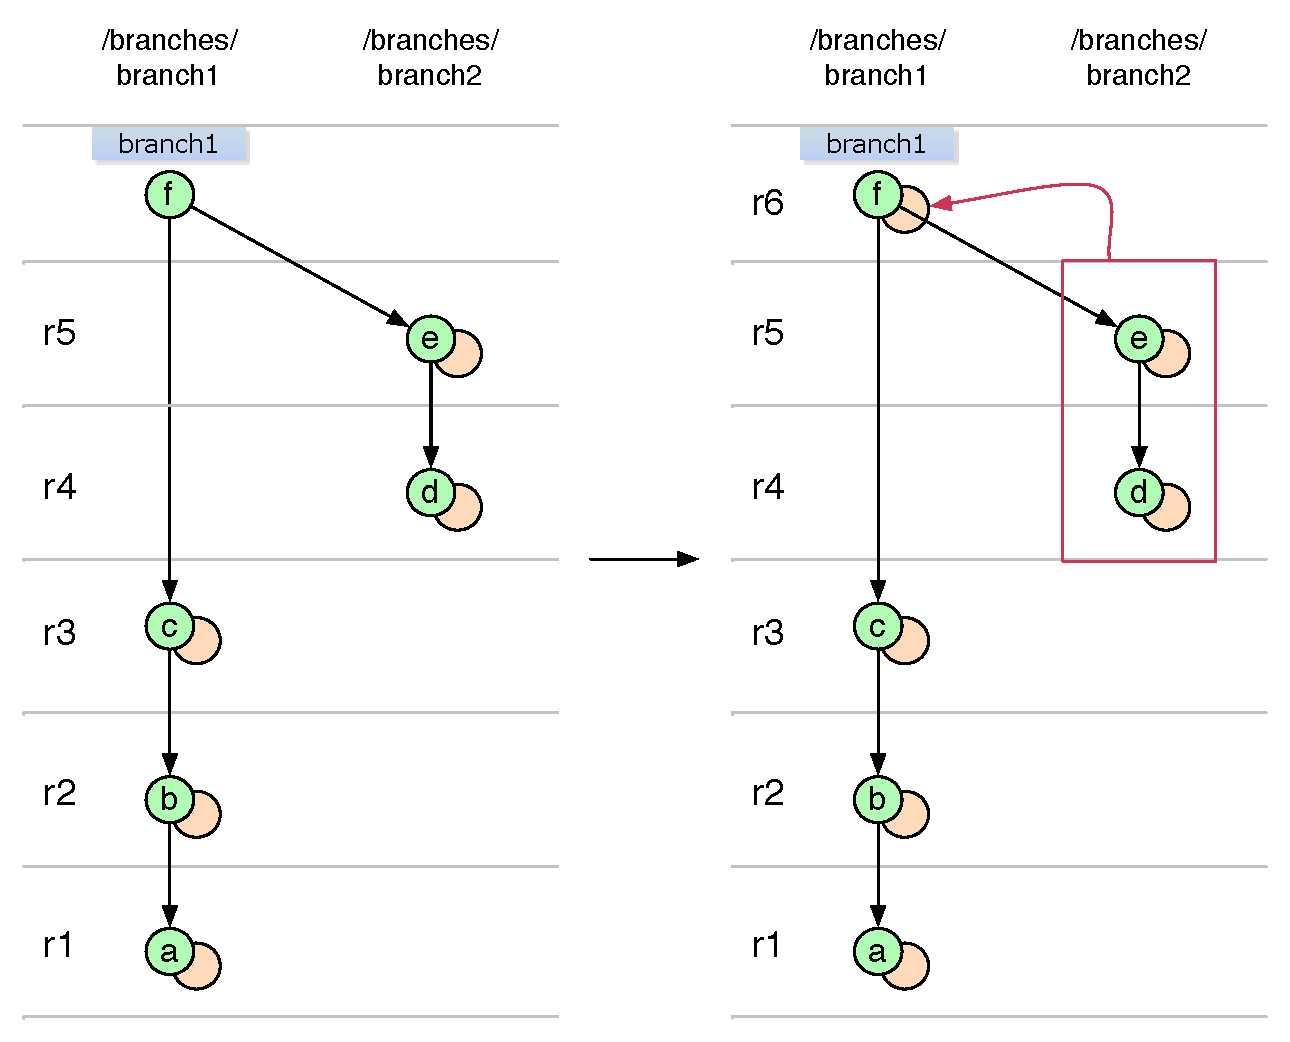
\includegraphics[width=\textwidth]{img/diagrams/simple_merge_branch_no_parent_git_to_svn.pdf}%
\captionof{figure}{Git merge commit being translated to the change of svn:mergeinfo property.}
\label{simple_merge_branch_no_parent_git_to_svn}%
\end{center}

It is natural to reverse this idea for Subversion to Git merge history translation. If revision r3 modified svn:mergeinfo property of branch branch1 that merge history of branch1 includes whole history of branch2, then merge commit should be created for that case. Diagrams \ref{simple_merge_svn_to_git} and \ref{simple_merge_branch_no_parent_svn_to_git} illustrate this approach.

\begin{center}
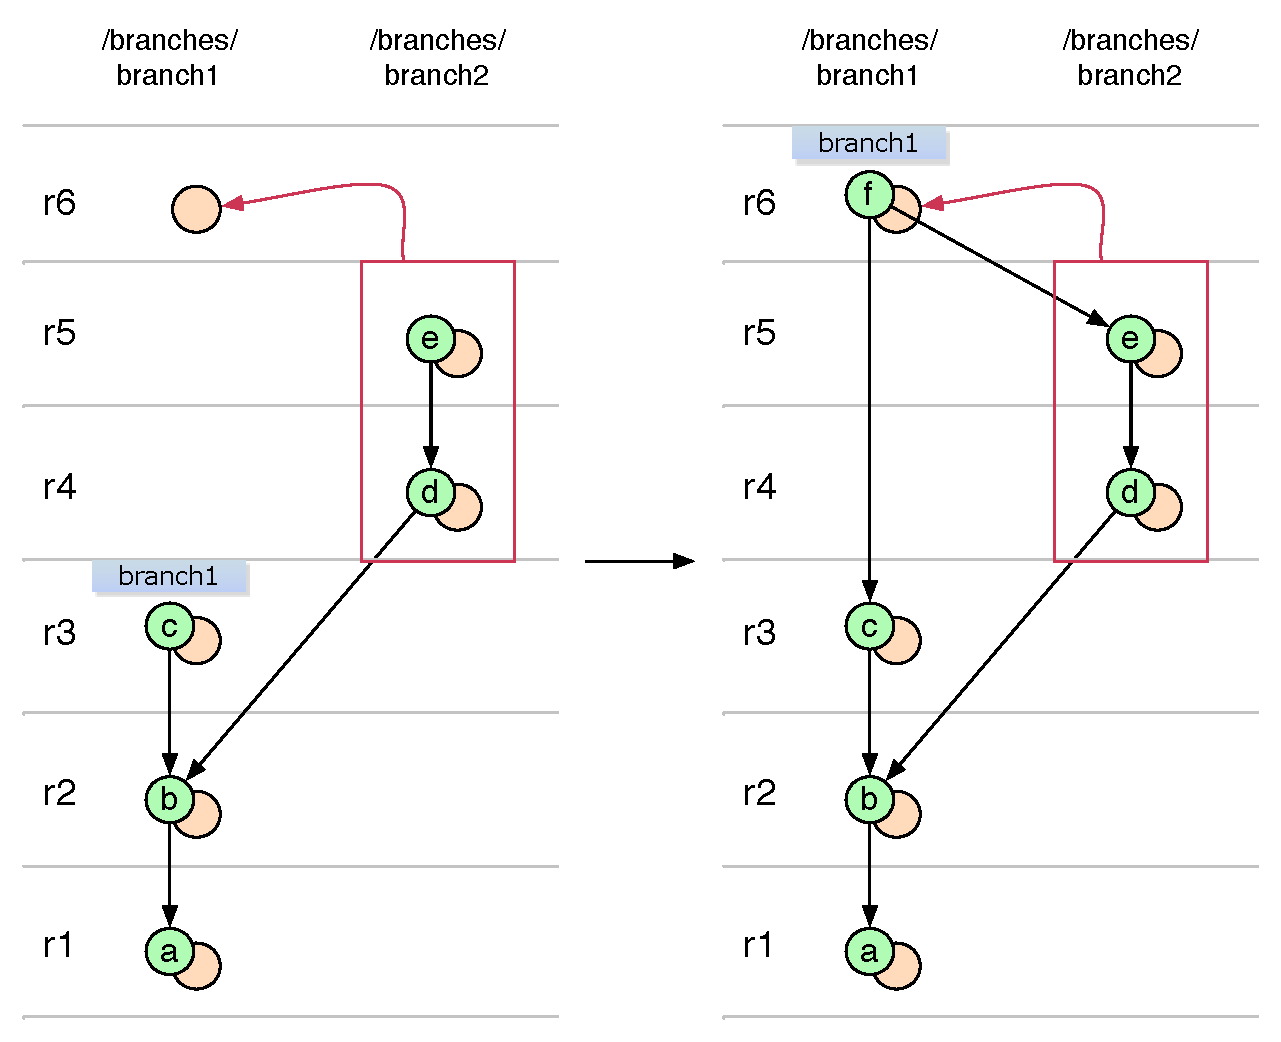
\includegraphics[width=\textwidth]{img/diagrams/simple_merge_svn_to_git.pdf}%
\captionof{figure}{svn:mergeinfo property change being translated into merge commit creation.}
\label{simple_merge_svn_to_git}%
\end{center}

\begin{center}
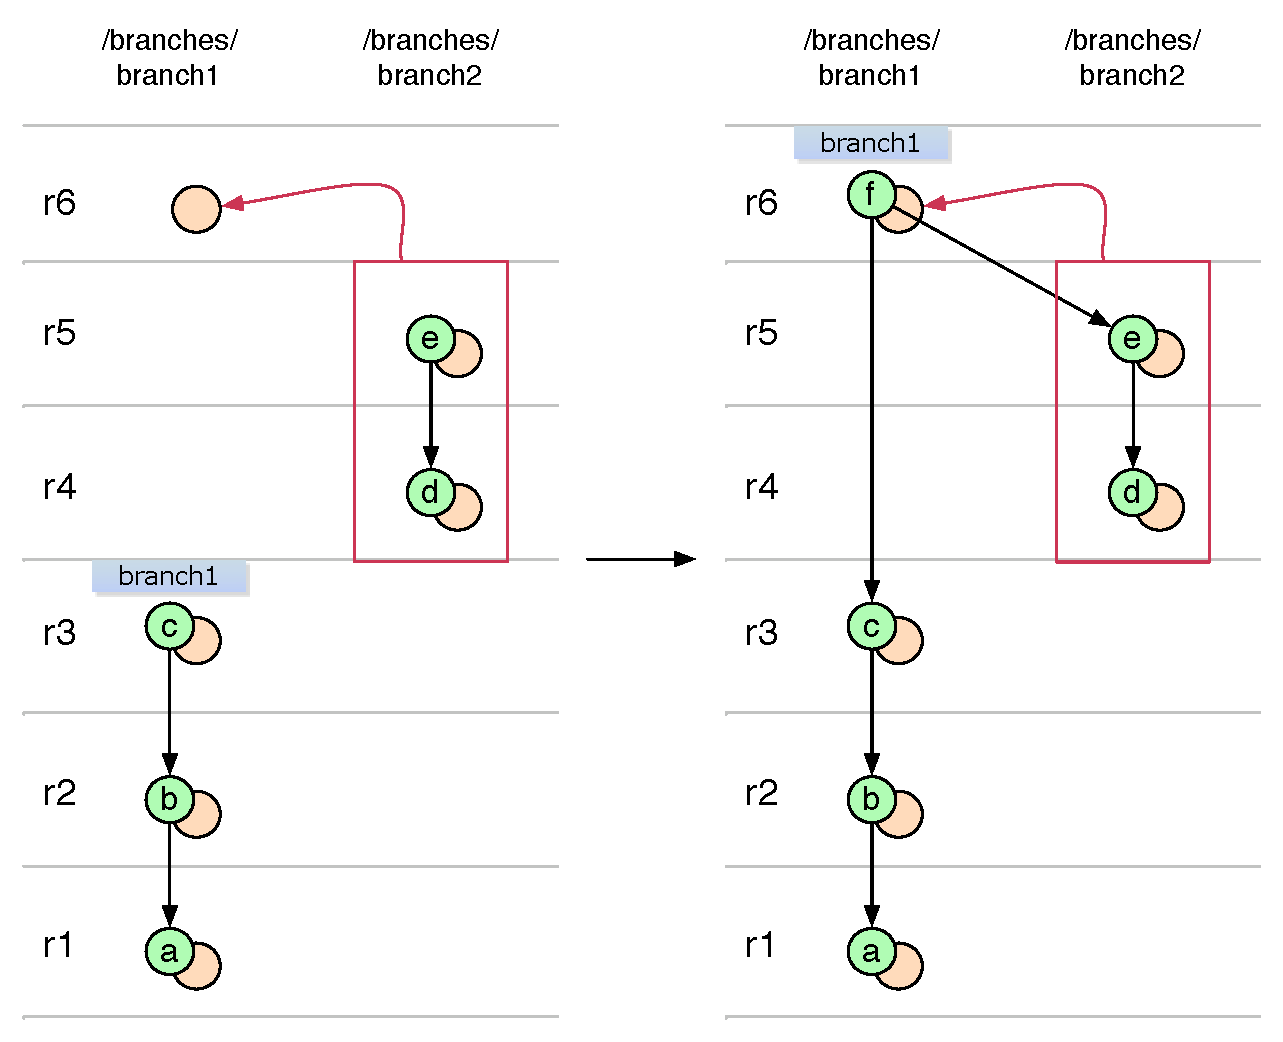
\includegraphics[width=\textwidth]{img/diagrams/simple_merge_branch_no_parent_svn_to_git.pdf}%
\captionof{figure}{svn:mergeinfo property change being translated into merge commit creation.}
\label{simple_merge_branch_no_parent_svn_to_git}%
\end{center}

\subsubsection{Cherry Pick}

Subversion tracks cherry-pick merges as well as merges of the whole branch history. Git doesn't support this kind of merges. Hence cherry-pick merge performed by Subversion user is translated as a new ordinary commit with corresponding changes at Git repository. This case depicted at diagram \ref{no_merge_commit_on_cherry_pick_svn_to_git}.

\begin{center}
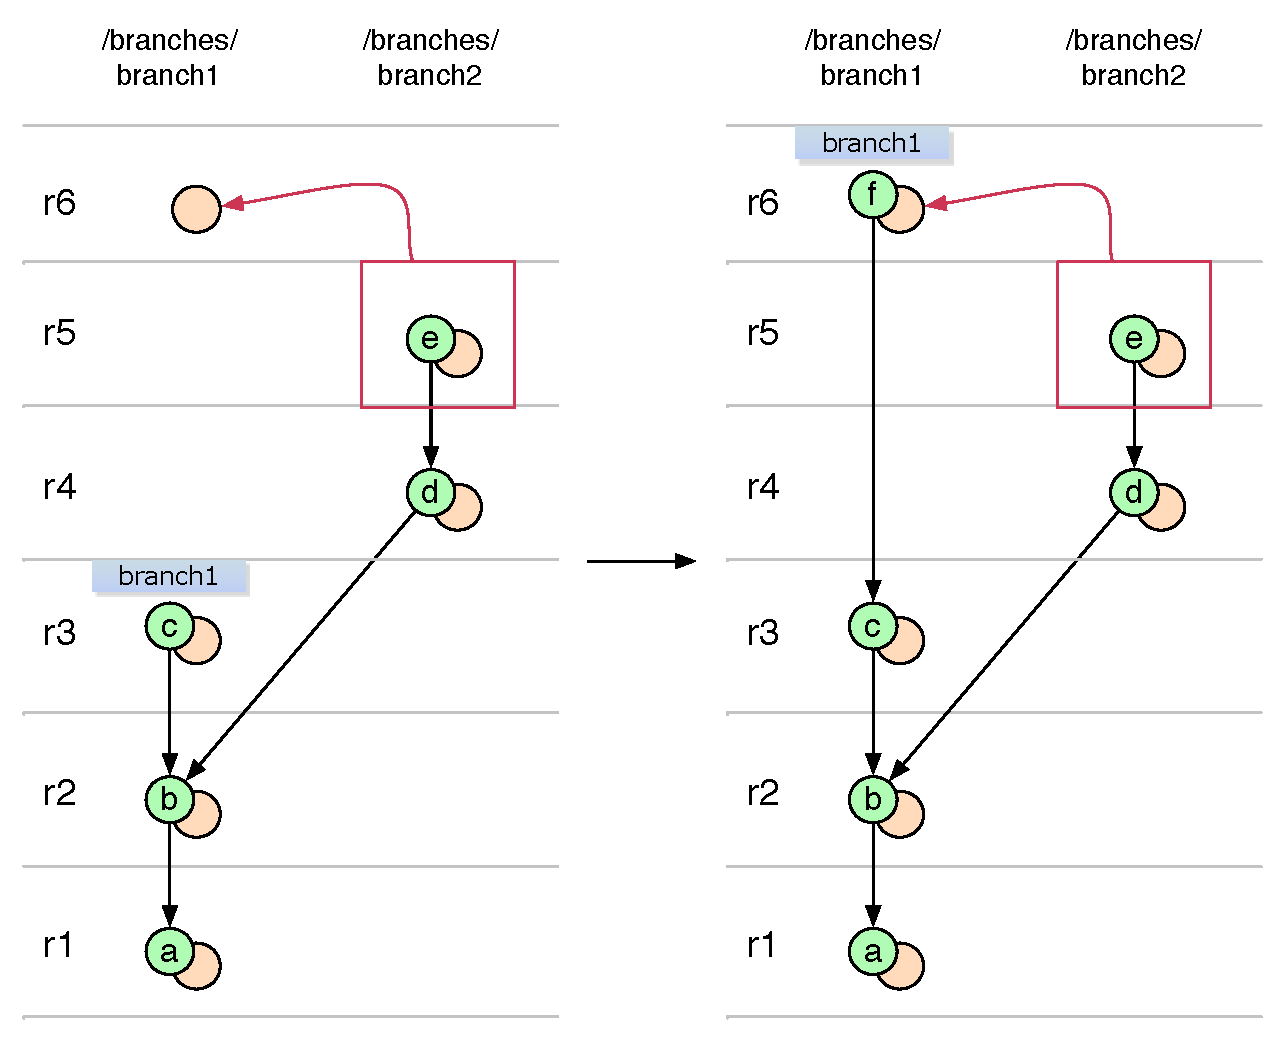
\includegraphics[width=\textwidth]{img/diagrams/no_merge_commit_on_cherry_pick_svn_to_git.pdf}%
\captionof{figure}{Cherry-pick merge being translated to ordinary commit.}
\label{no_merge_commit_on_cherry_pick_svn_to_git}%
\end{center}

A sequence of cherry-pick revisions may lead the history of certain branch to the state when it includes the history of another branch as merge history. This scenario is depicted at diagrams \ref{merge_commit_on_double_cherry_pick_svn_to_git} and \ref{merge_commit_on_double_cherry_pick_branch_no_parent_svn_to_git}.

\begin{center}
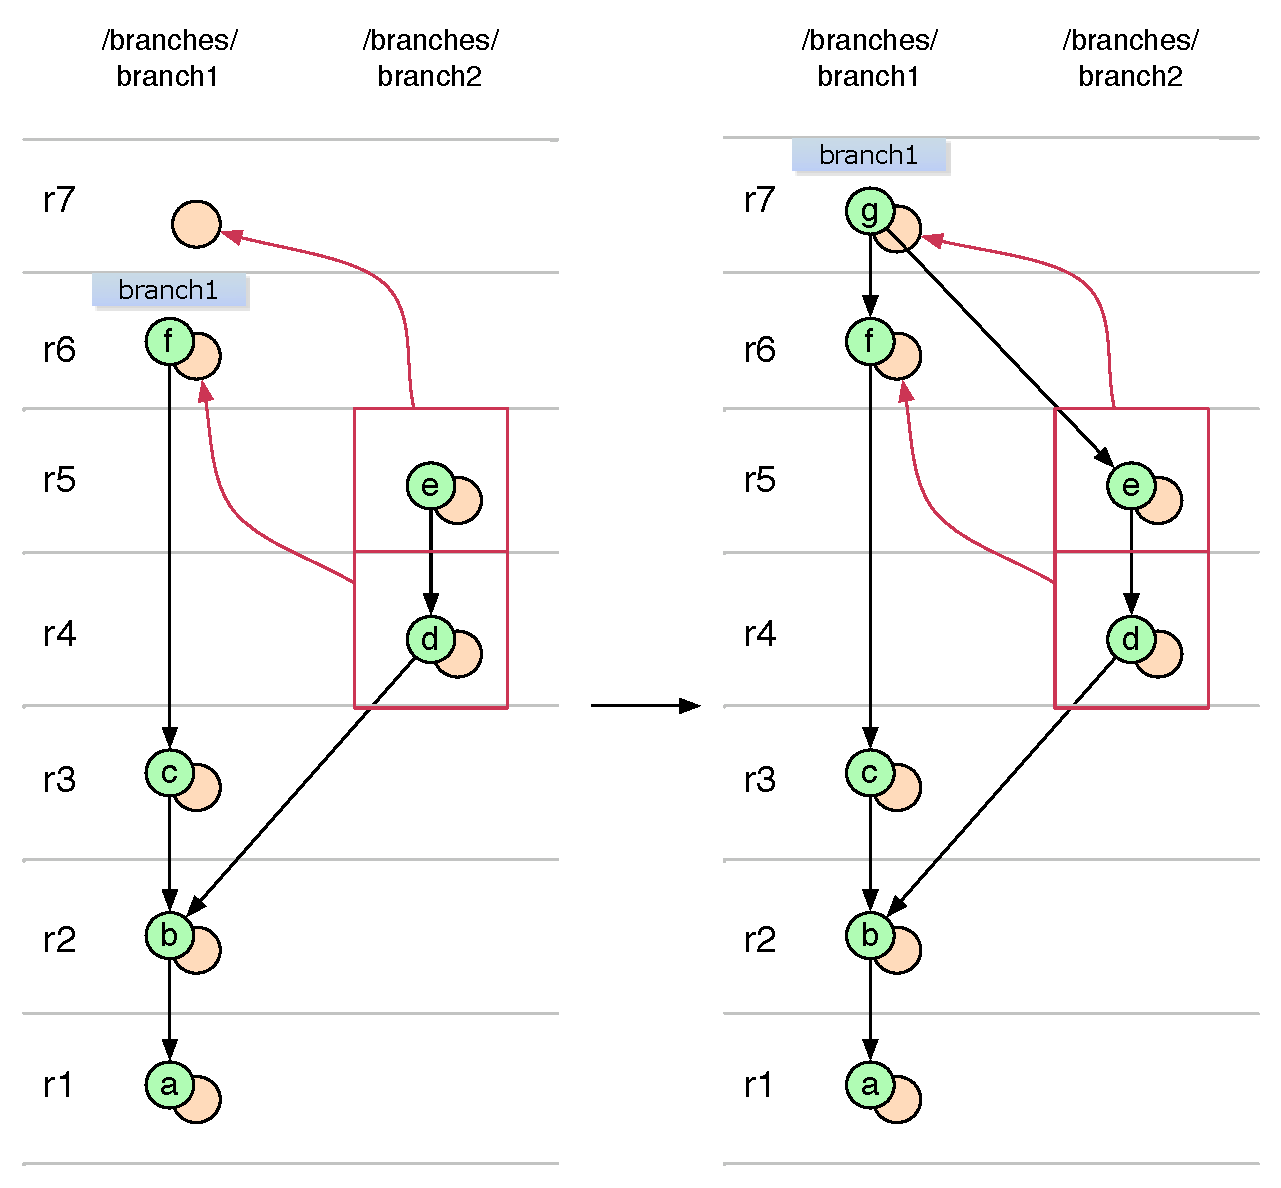
\includegraphics[width=\textwidth]{img/diagrams/merge_commit_on_double_cherry_pick_svn_to_git.pdf}%
\captionof{figure}{A sequence of cherry-pick merges being translated to merge commit.}
\label{merge_commit_on_double_cherry_pick_svn_to_git}%
\end{center}

\begin{center}
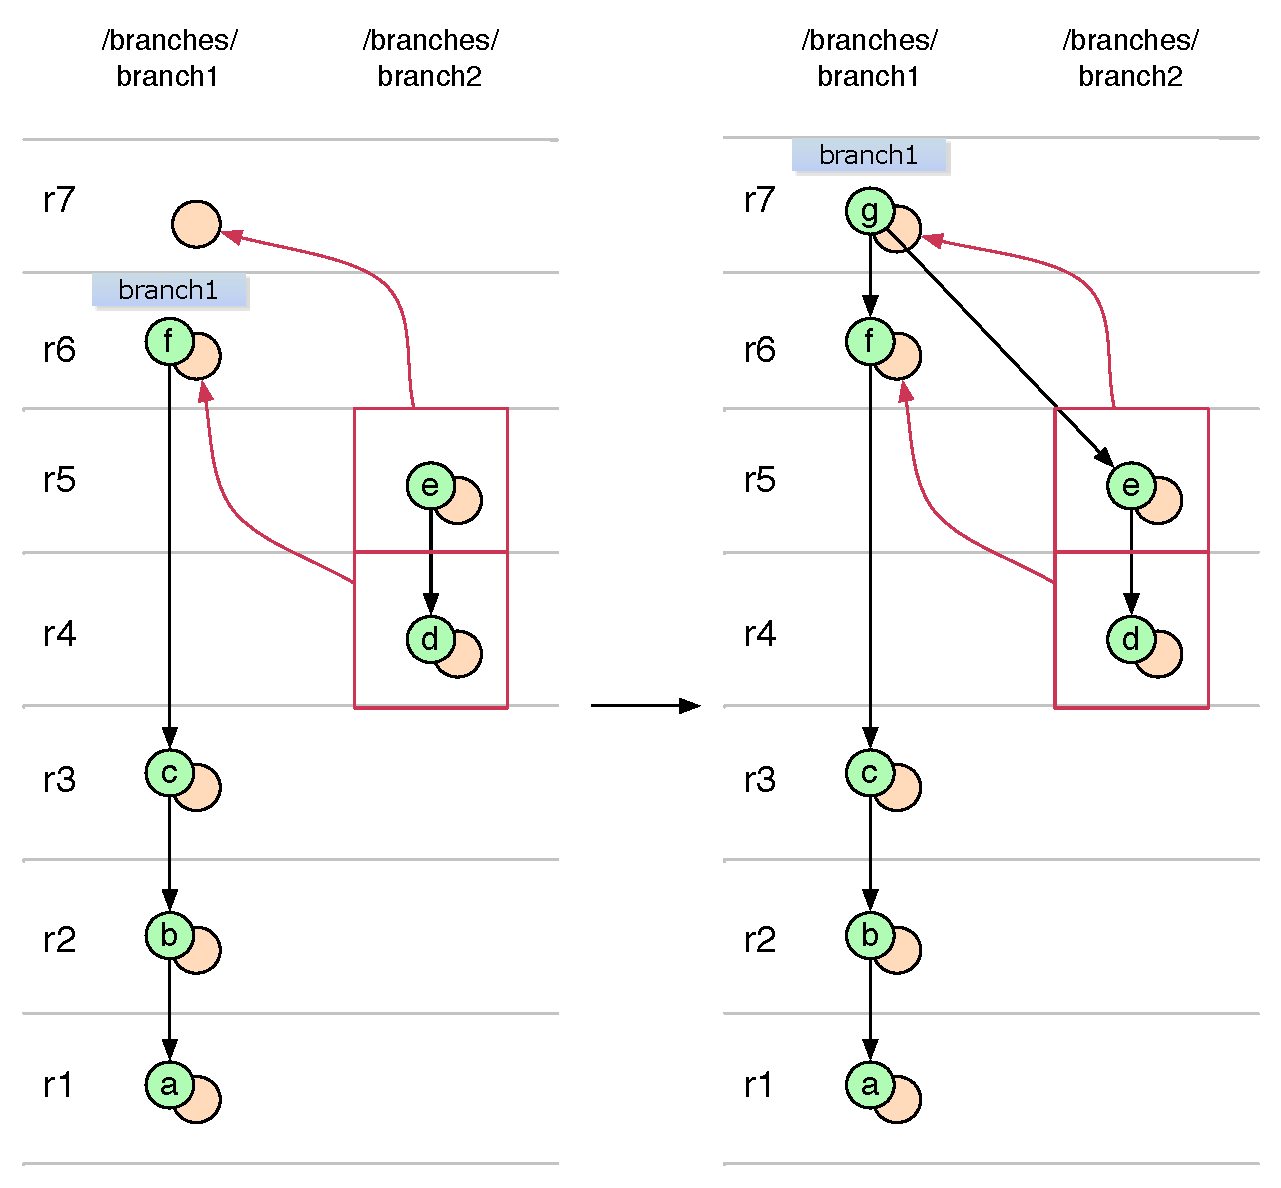
\includegraphics[width=\textwidth]{img/diagrams/merge_commit_on_double_cherry_pick_branch_no_parent_svn_to_git.pdf}%
\captionof{figure}{A sequence of cherry-pick merges being translated to merge commit.}
\label{merge_commit_on_double_cherry_pick_branch_no_parent_svn_to_git}%
\end{center}

\subsubsection{Shelve Branches}

Git user is able to push an arbitrary number of commits at once. These commits may include merges. Assuming the scenario depicted at diagram \ref{boat_merge_named_shelve_git_to_svn}, Translator is able to determine the name of the branch merged into branch branch1 at commit \emph{f}.

\begin{center}
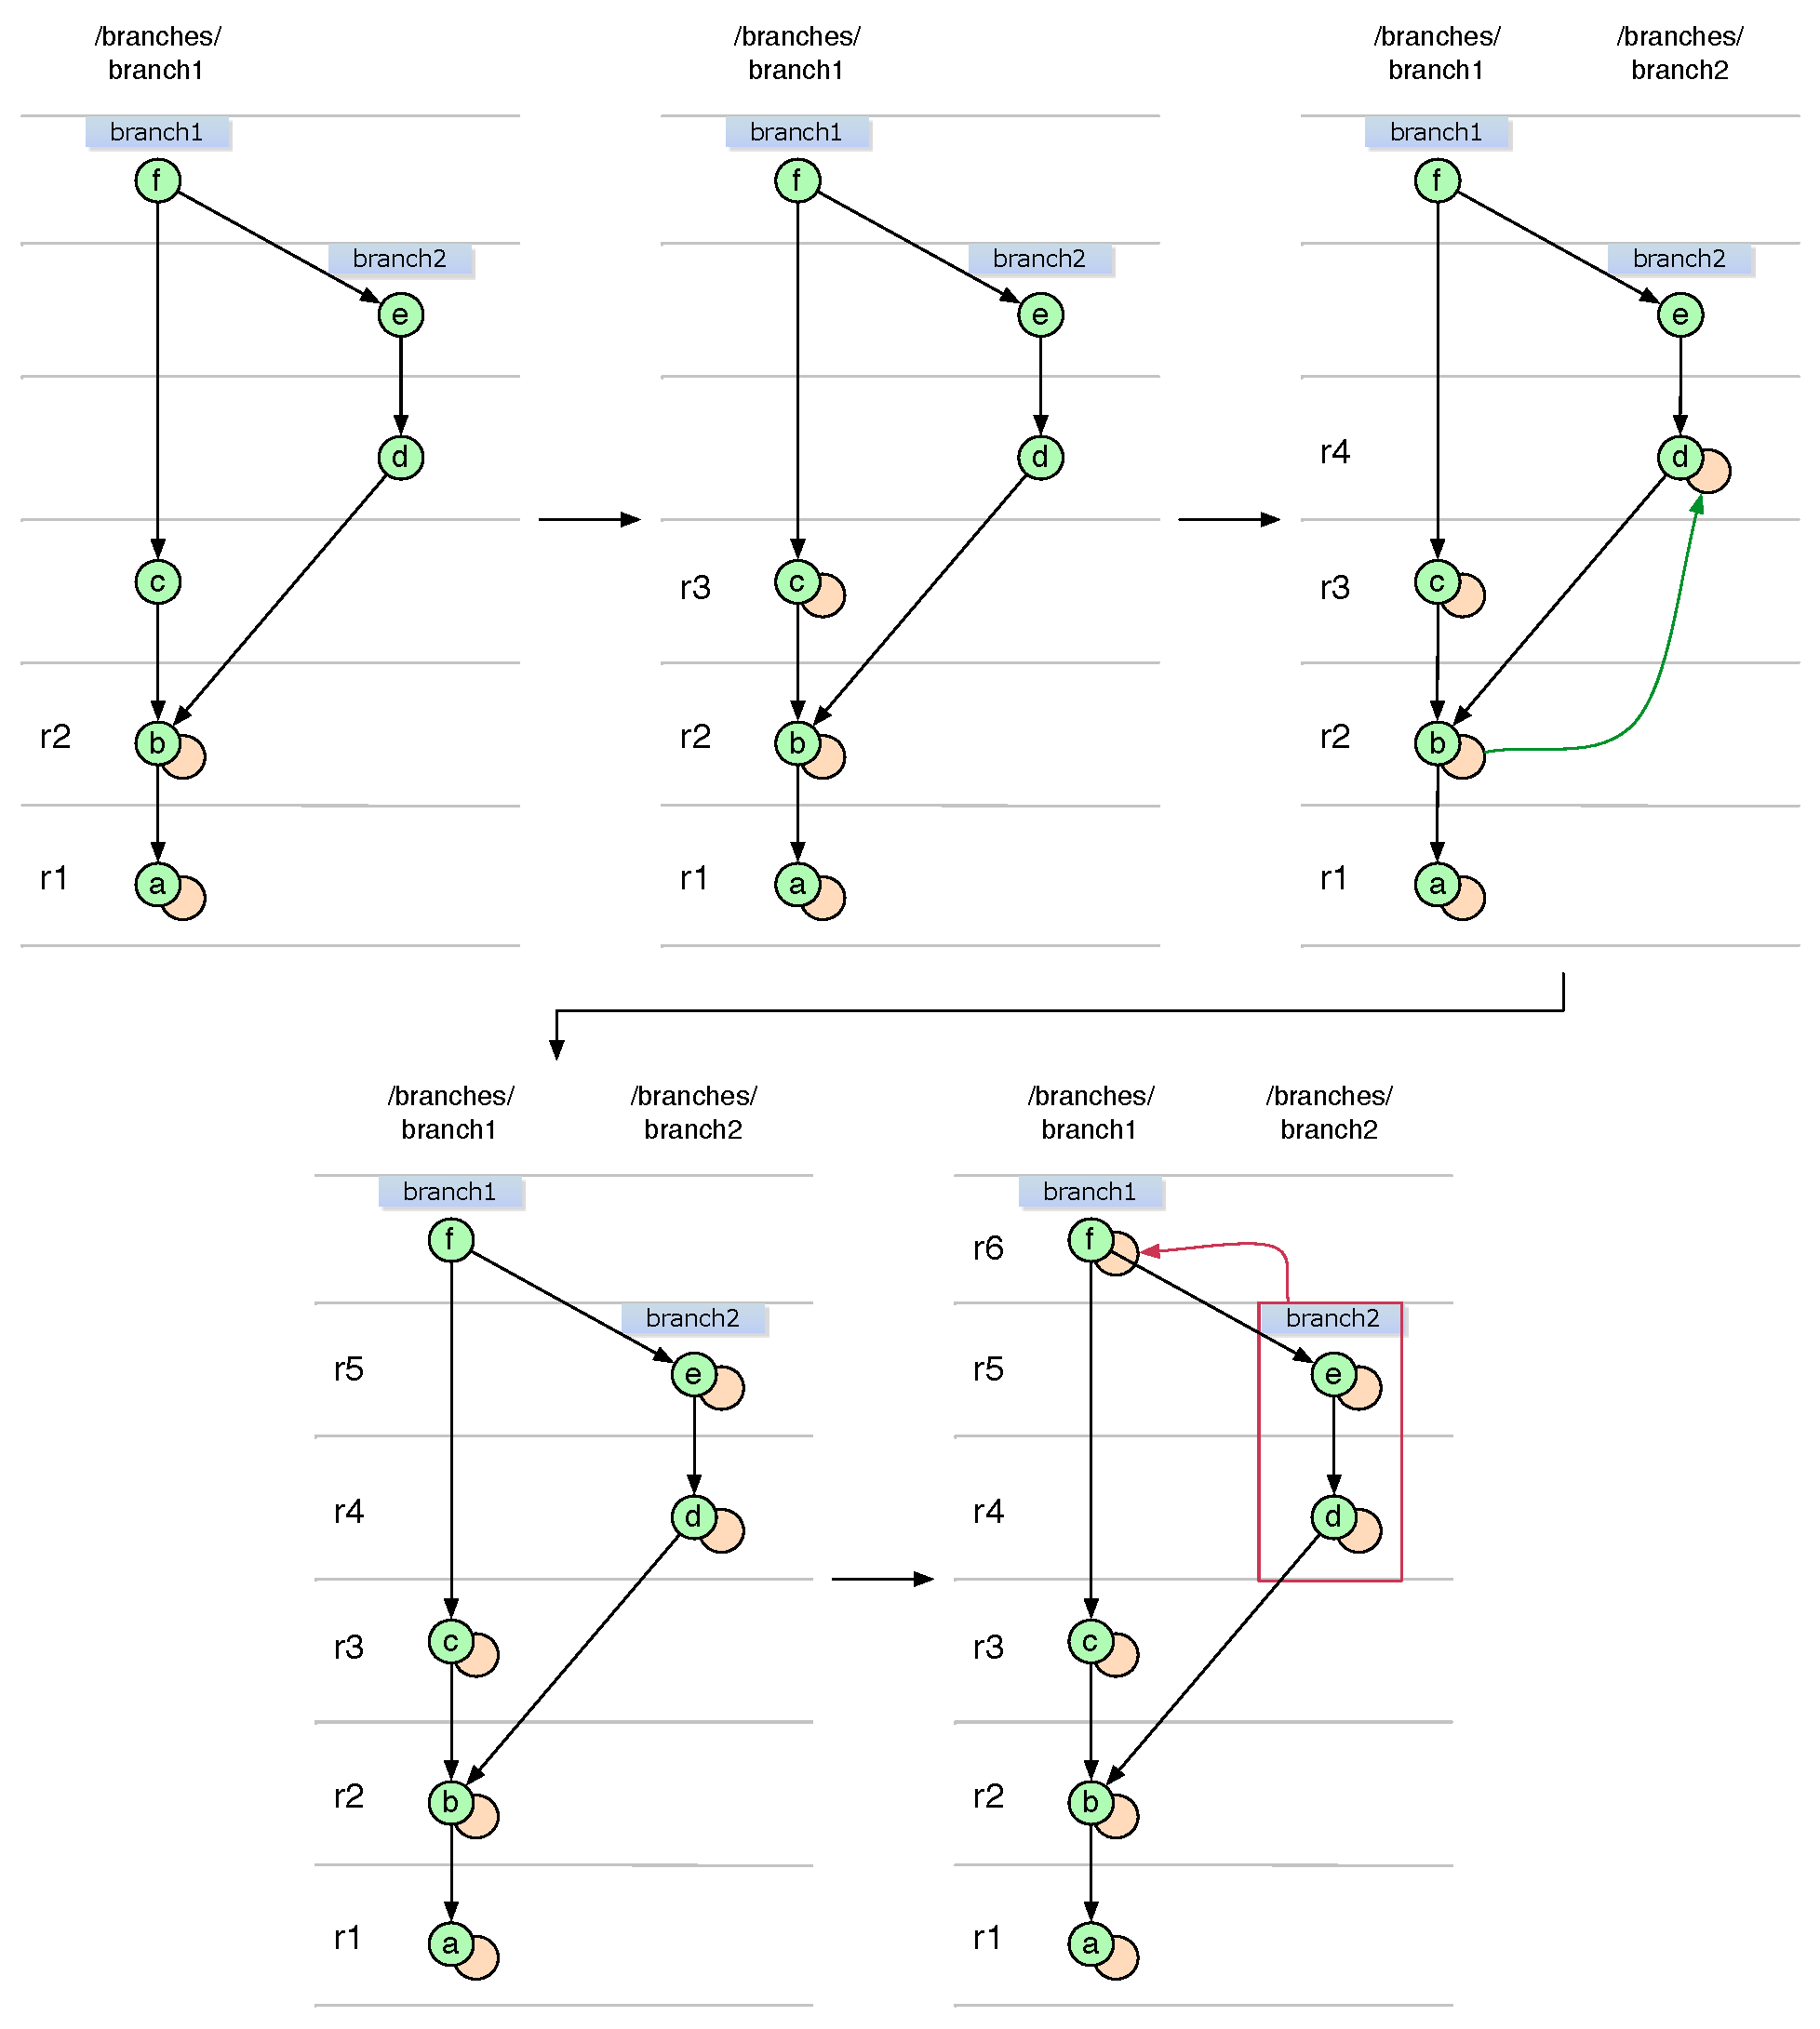
\includegraphics[width=\textwidth]{img/diagrams/boat_merge_named_shelve_git_to_svn.pdf}%
\captionof{figure}{Merge of Git branch which is available from another branch being translated to a sequence of Subversion revisions.}
\label{boat_merge_named_shelve_git_to_svn}%
\end{center}

Assuming the scenario depicted at diagram \ref{boat_merge_shelve_is_normal_branch_git_to_svn}, Translator is able to determine the name of the branch merged into branch branch1 by following first parent commits from branch2 reference.

\begin{center}
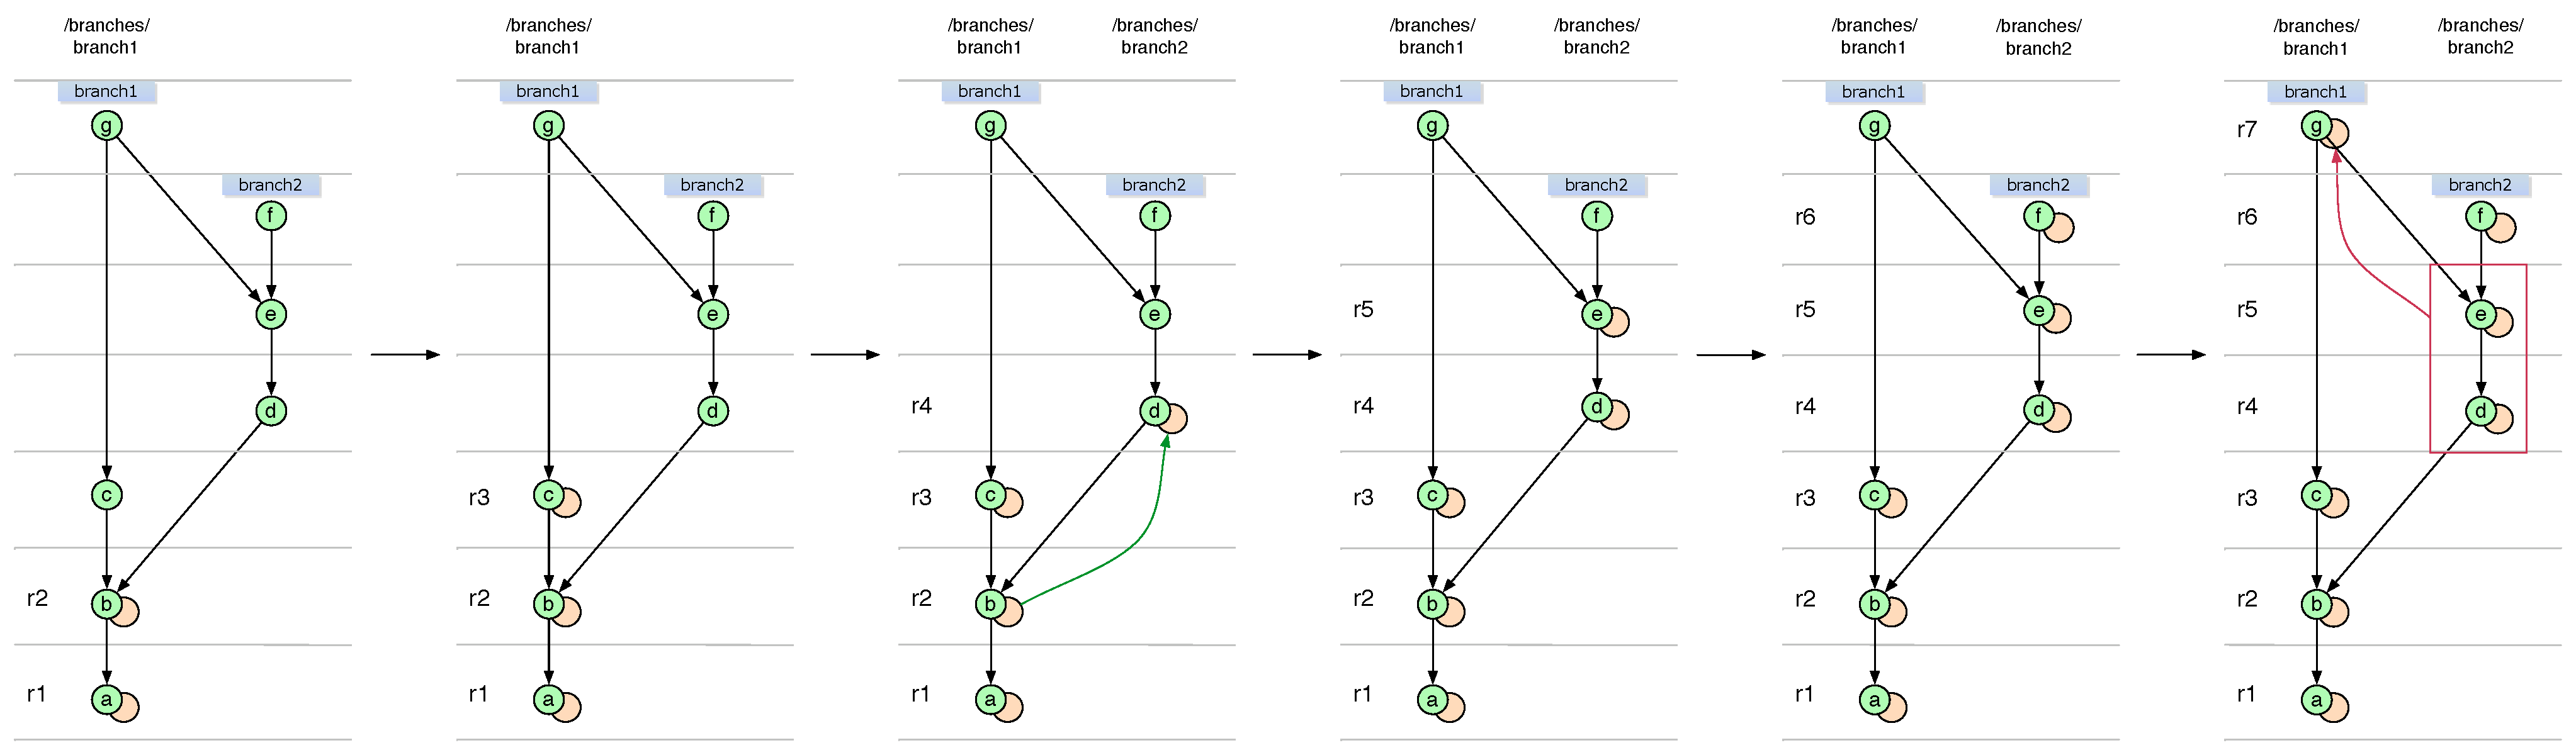
\includegraphics[width=\textwidth]{img/diagrams/boat_merge_shelve_is_normal_branch_git_to_svn.pdf}%
\captionof{figure}{Merge of Git branch which is available from another branch being translated to a sequence of Subversion revisions.}
\label{boat_merge_shelve_is_normal_branch_git_to_svn}%
\end{center}

There are scenarios when Translator is not able to determine the name of merged branch, see diagram \ref{boat_merge_git_to_svn}. For that case synthetic shelve branch created. Translator use specific namespace /shelves/ and name of person created the first commit on the shelve to generate the name of the branch. As soon as merge is performed the shelve is deleted.

\begin{center}
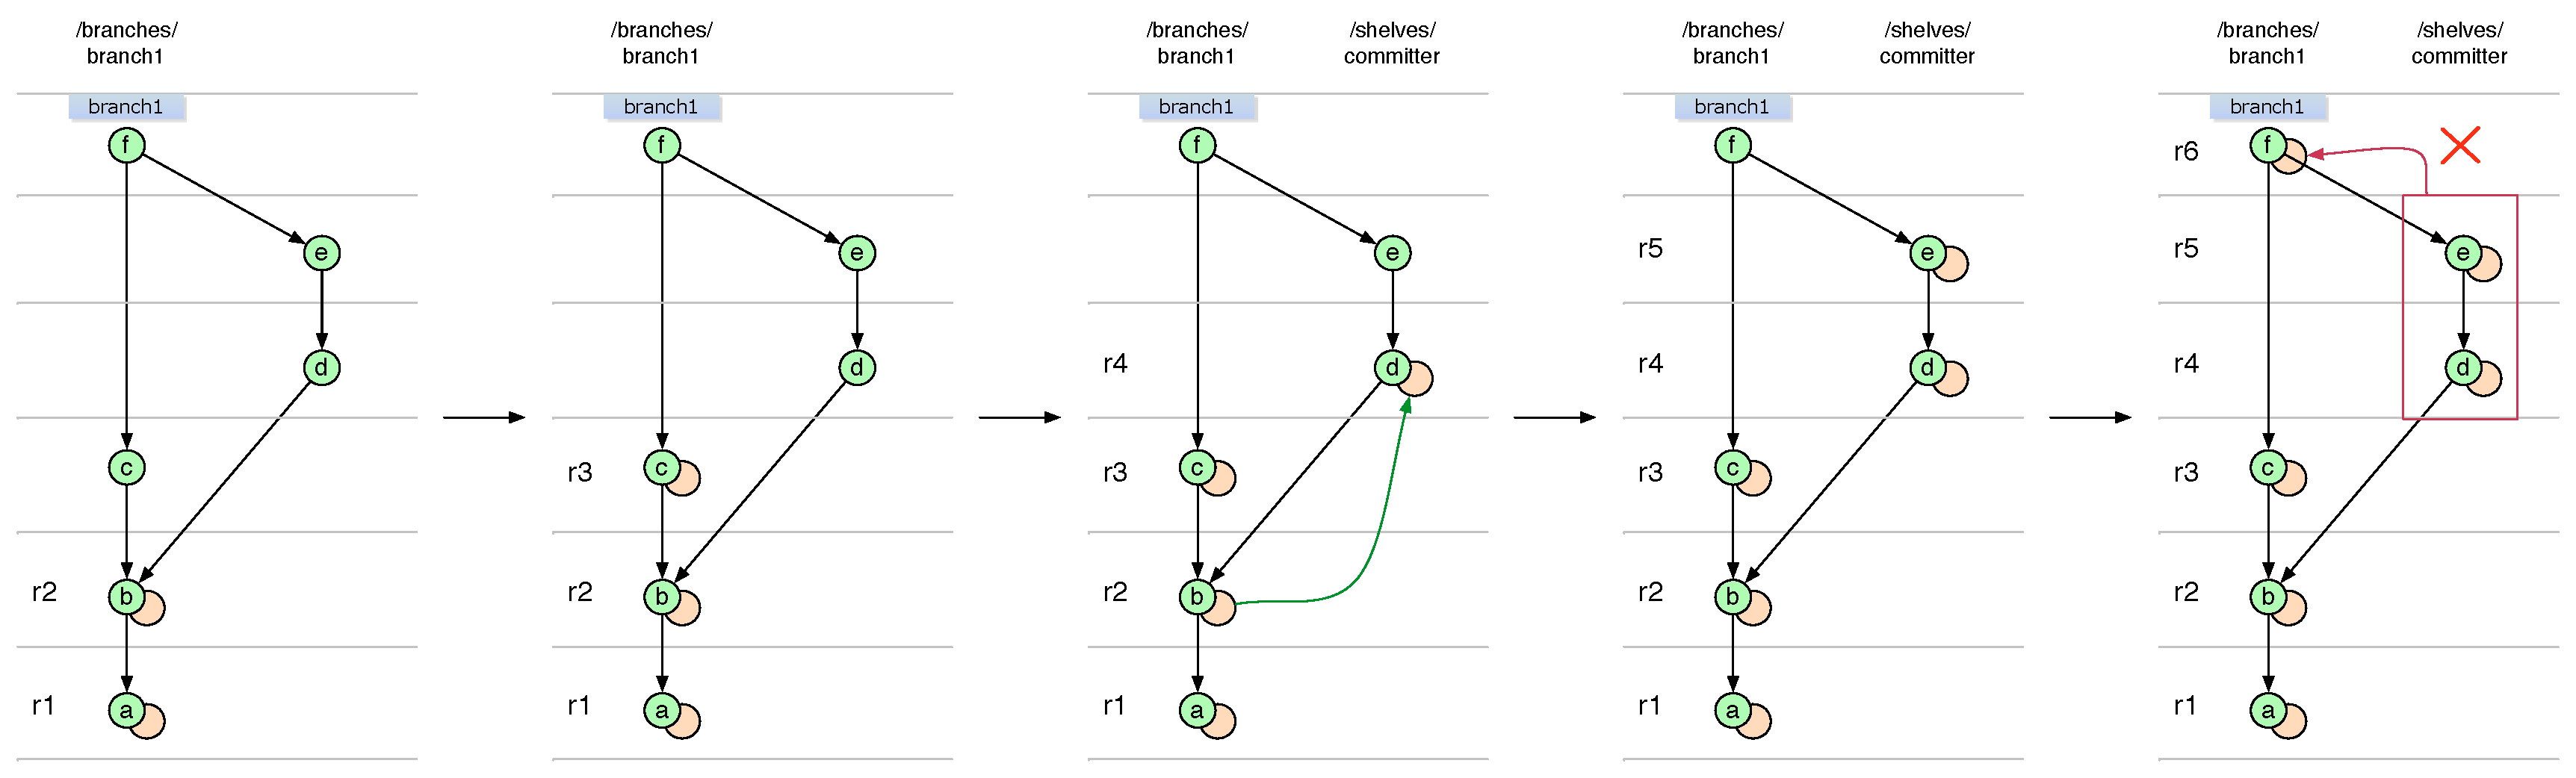
\includegraphics[width=\textwidth]{img/diagrams/boat_merge_git_to_svn.pdf}%
\captionof{figure}{Merge of unnamed Git branch being translated to a sequence of Subversion revisions.}
\label{boat_merge_git_to_svn}%
\end{center}

\subsubsection{Shelve Linearization}

It's common use case when multiple users performed modification and then merged all together at the main development branch of the remote repository. For this scenario every user's branch becomes a shelve. For Subversion users it is not a typical workflow, they are accustomed to have linear history of changes produced by different users.
\\\\
As an experimental feature for that case we introduce a shelve linearization approach depicted at diagram \ref{boat_merge_keep_history_linear_git_to_svn}.
\begin{center}
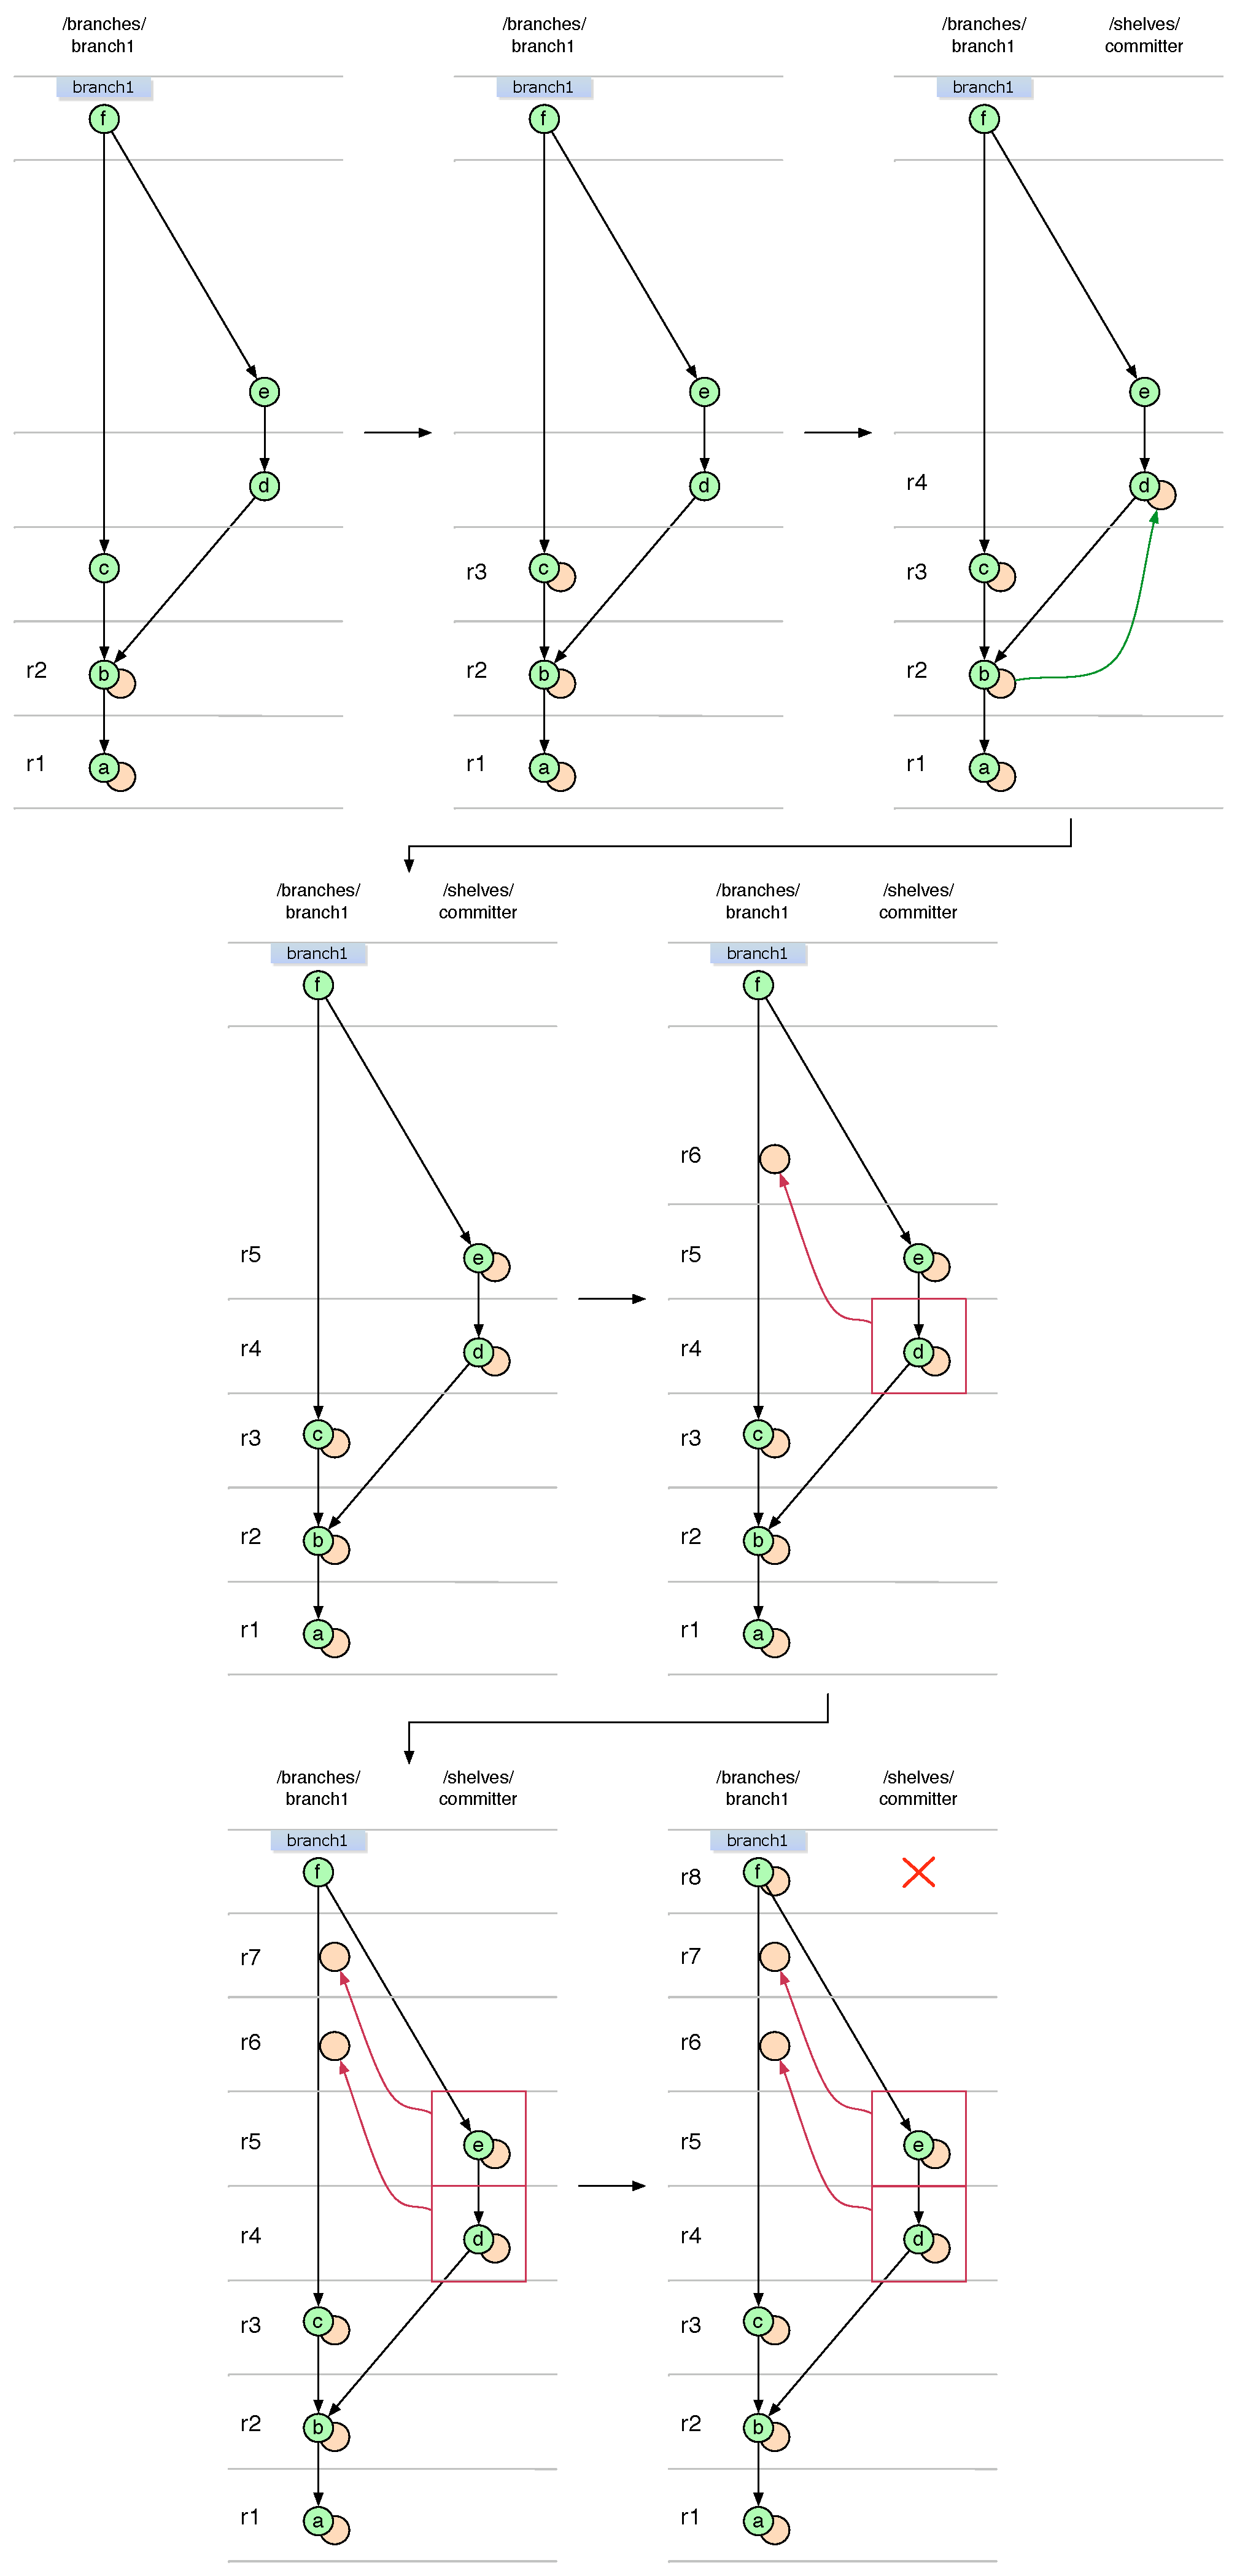
\includegraphics[width=\textwidth]{img/diagrams/boat_merge_keep_history_linear_git_to_svn.pdf}%
\captionof{figure}{Merge of Git branch which is available from another branch being translated to a sequence of Subversion revisions.}
\label{boat_merge_keep_history_linear_git_to_svn}%
\end{center}

If commit \emph{c} and a couple of commits \emph{d} and \emph{c} modified not intersecting set of files, then it is possible to imitate linear history for branch branch1. For that purpose Translator creates three revisions r6, r7, r8 instead of a single revision that would be mapped to merge commit \emph{f}.
\\\\
For every commit at shelve Translator generates a revision with synthetic cherry-pick merge of the revision mapped to this commit. Finally revision r8 is the revision corresponding to commit \emph{f} and also it has the history of the shelve within svn:mergeinfo property. Hence mapping commit \emph{f} to revision r8 is valid. Having these revisions at branch branch1 Subversion users see history of branch branch1 linear.
\\\\
Shelve linearization has a few drawbacks:
\begin{enumerate}
\compactlist
	\item Main branch and shelve must not modify the same file, otherwise the approach is not applicable.
	\item At revisions r7 and r8 there could appear build failures since at this revision branch1 state is generated by Translator with no additional checks.
	\item This approach violates commits to revision mapping, since emph{f} commit should be mapped to a sequence of revision r6, r7 and r8 instead of one single revision. It needs an extension of suggested commit to revision mapping.
\end{enumerate}

Shelve linearization could be applied to any branch to keep history linear. But shelve is the most common use case.

\subsubsection{Nested Merge}

\begin{center}
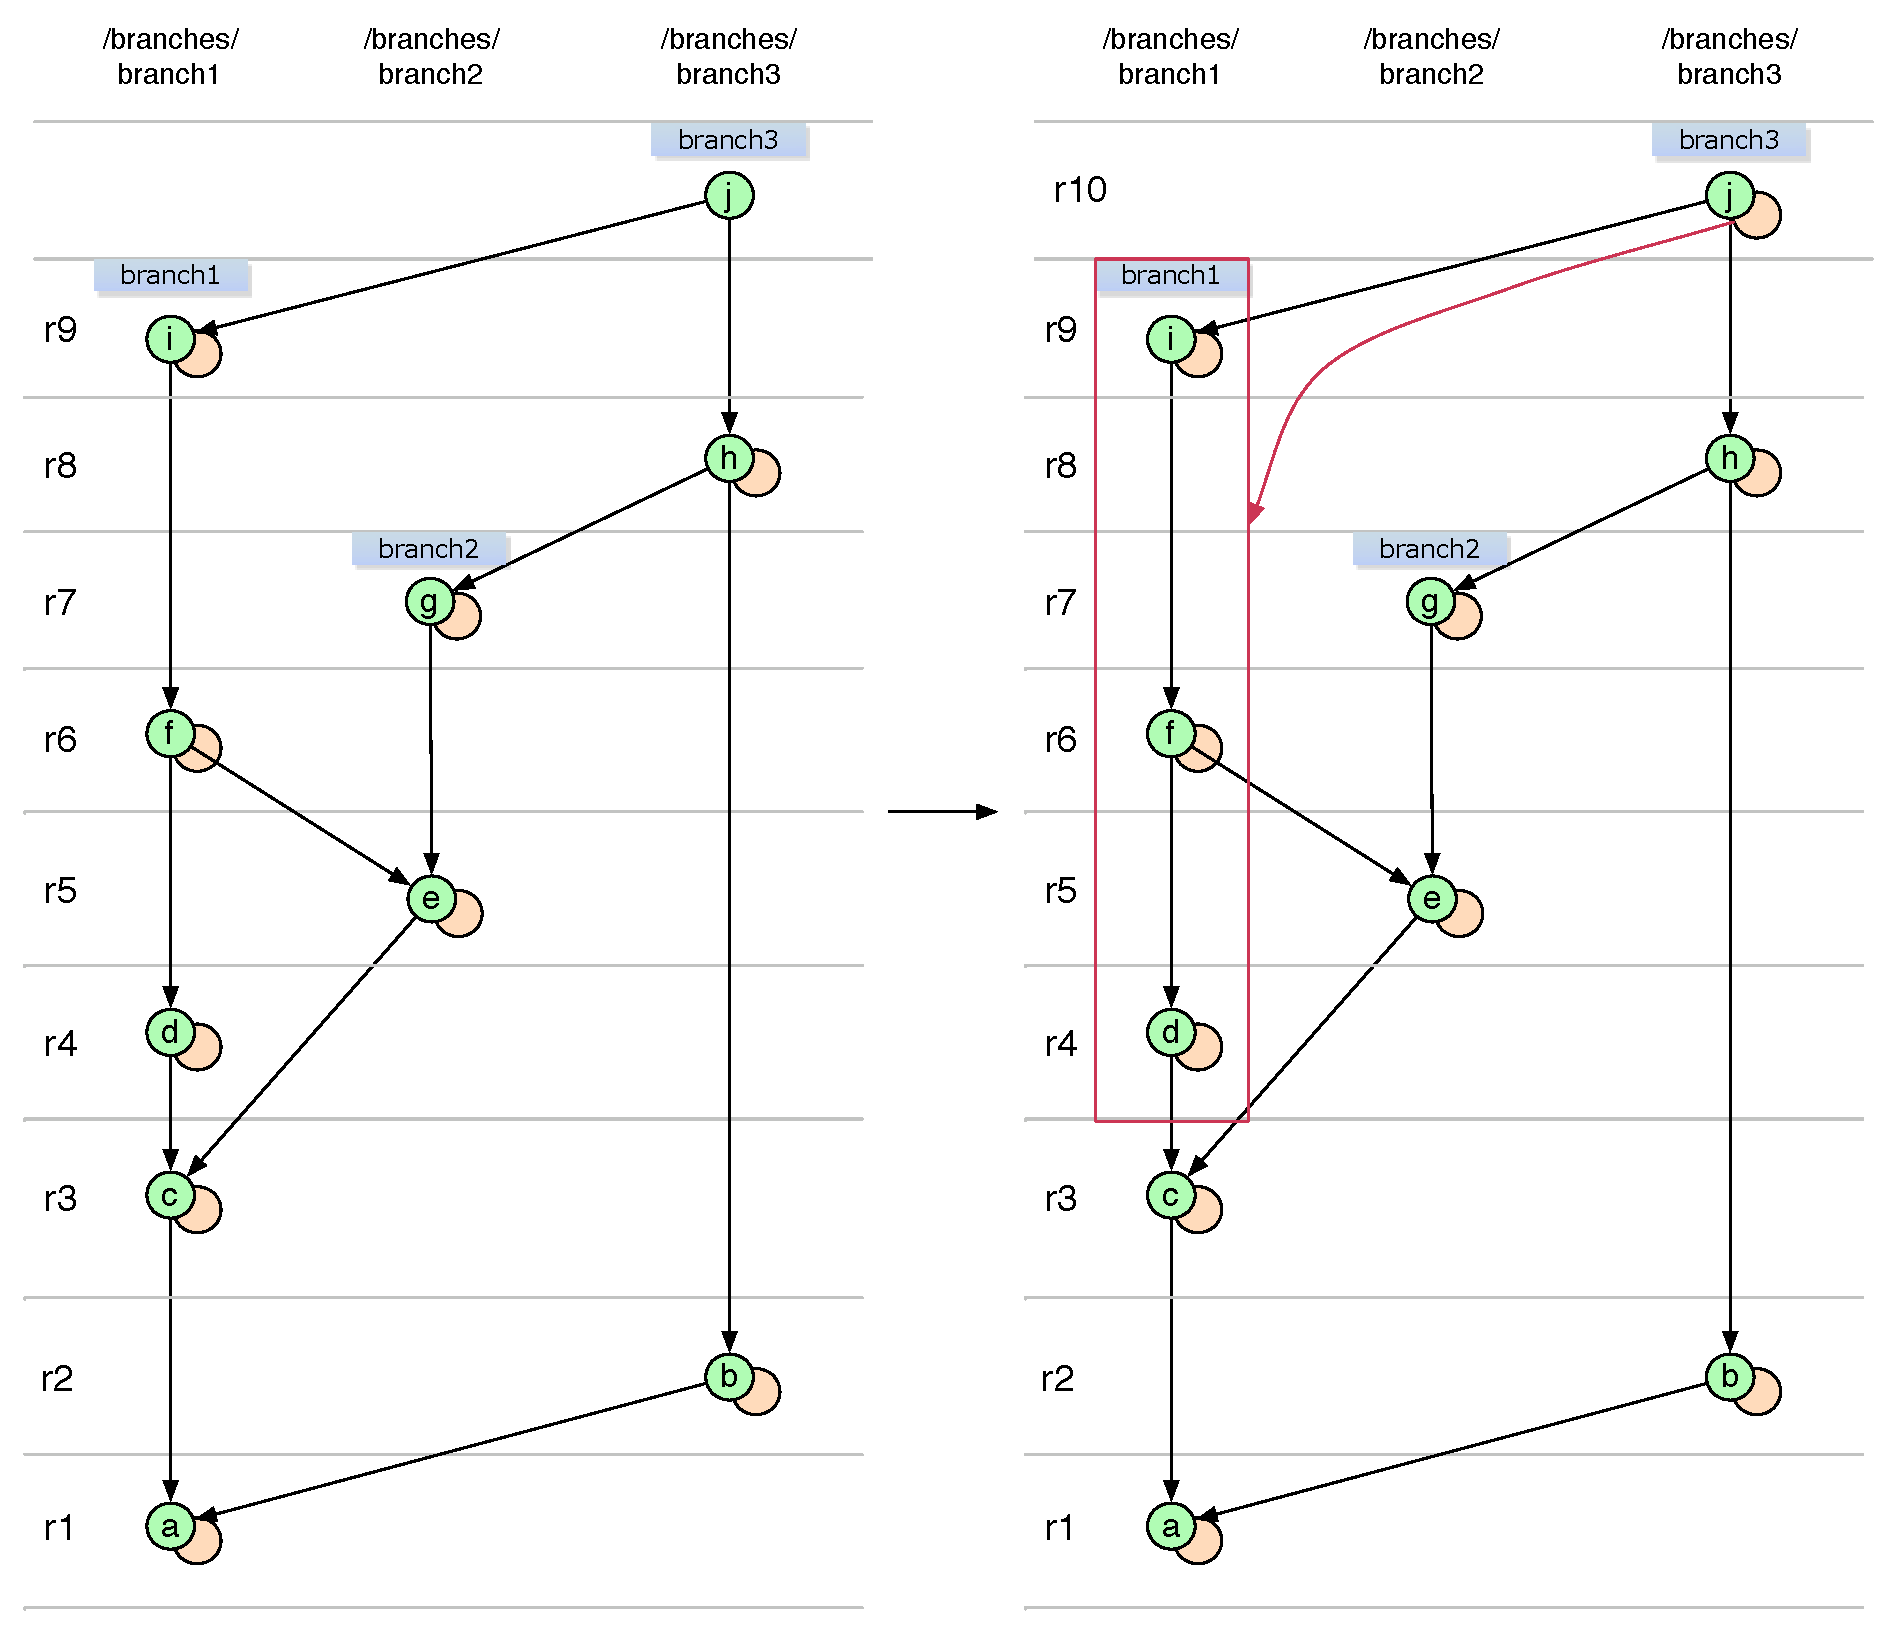
\includegraphics[width=\textwidth]{img/diagrams/merge_sequence_git_to_svn.pdf}%
\captionof{figure}{Merge of Git branch which is available from another branch being translated to a sequence of Subversion revisions.}
\label{merge_sequence_git_to_svn}%
\end{center}

\begin{center}
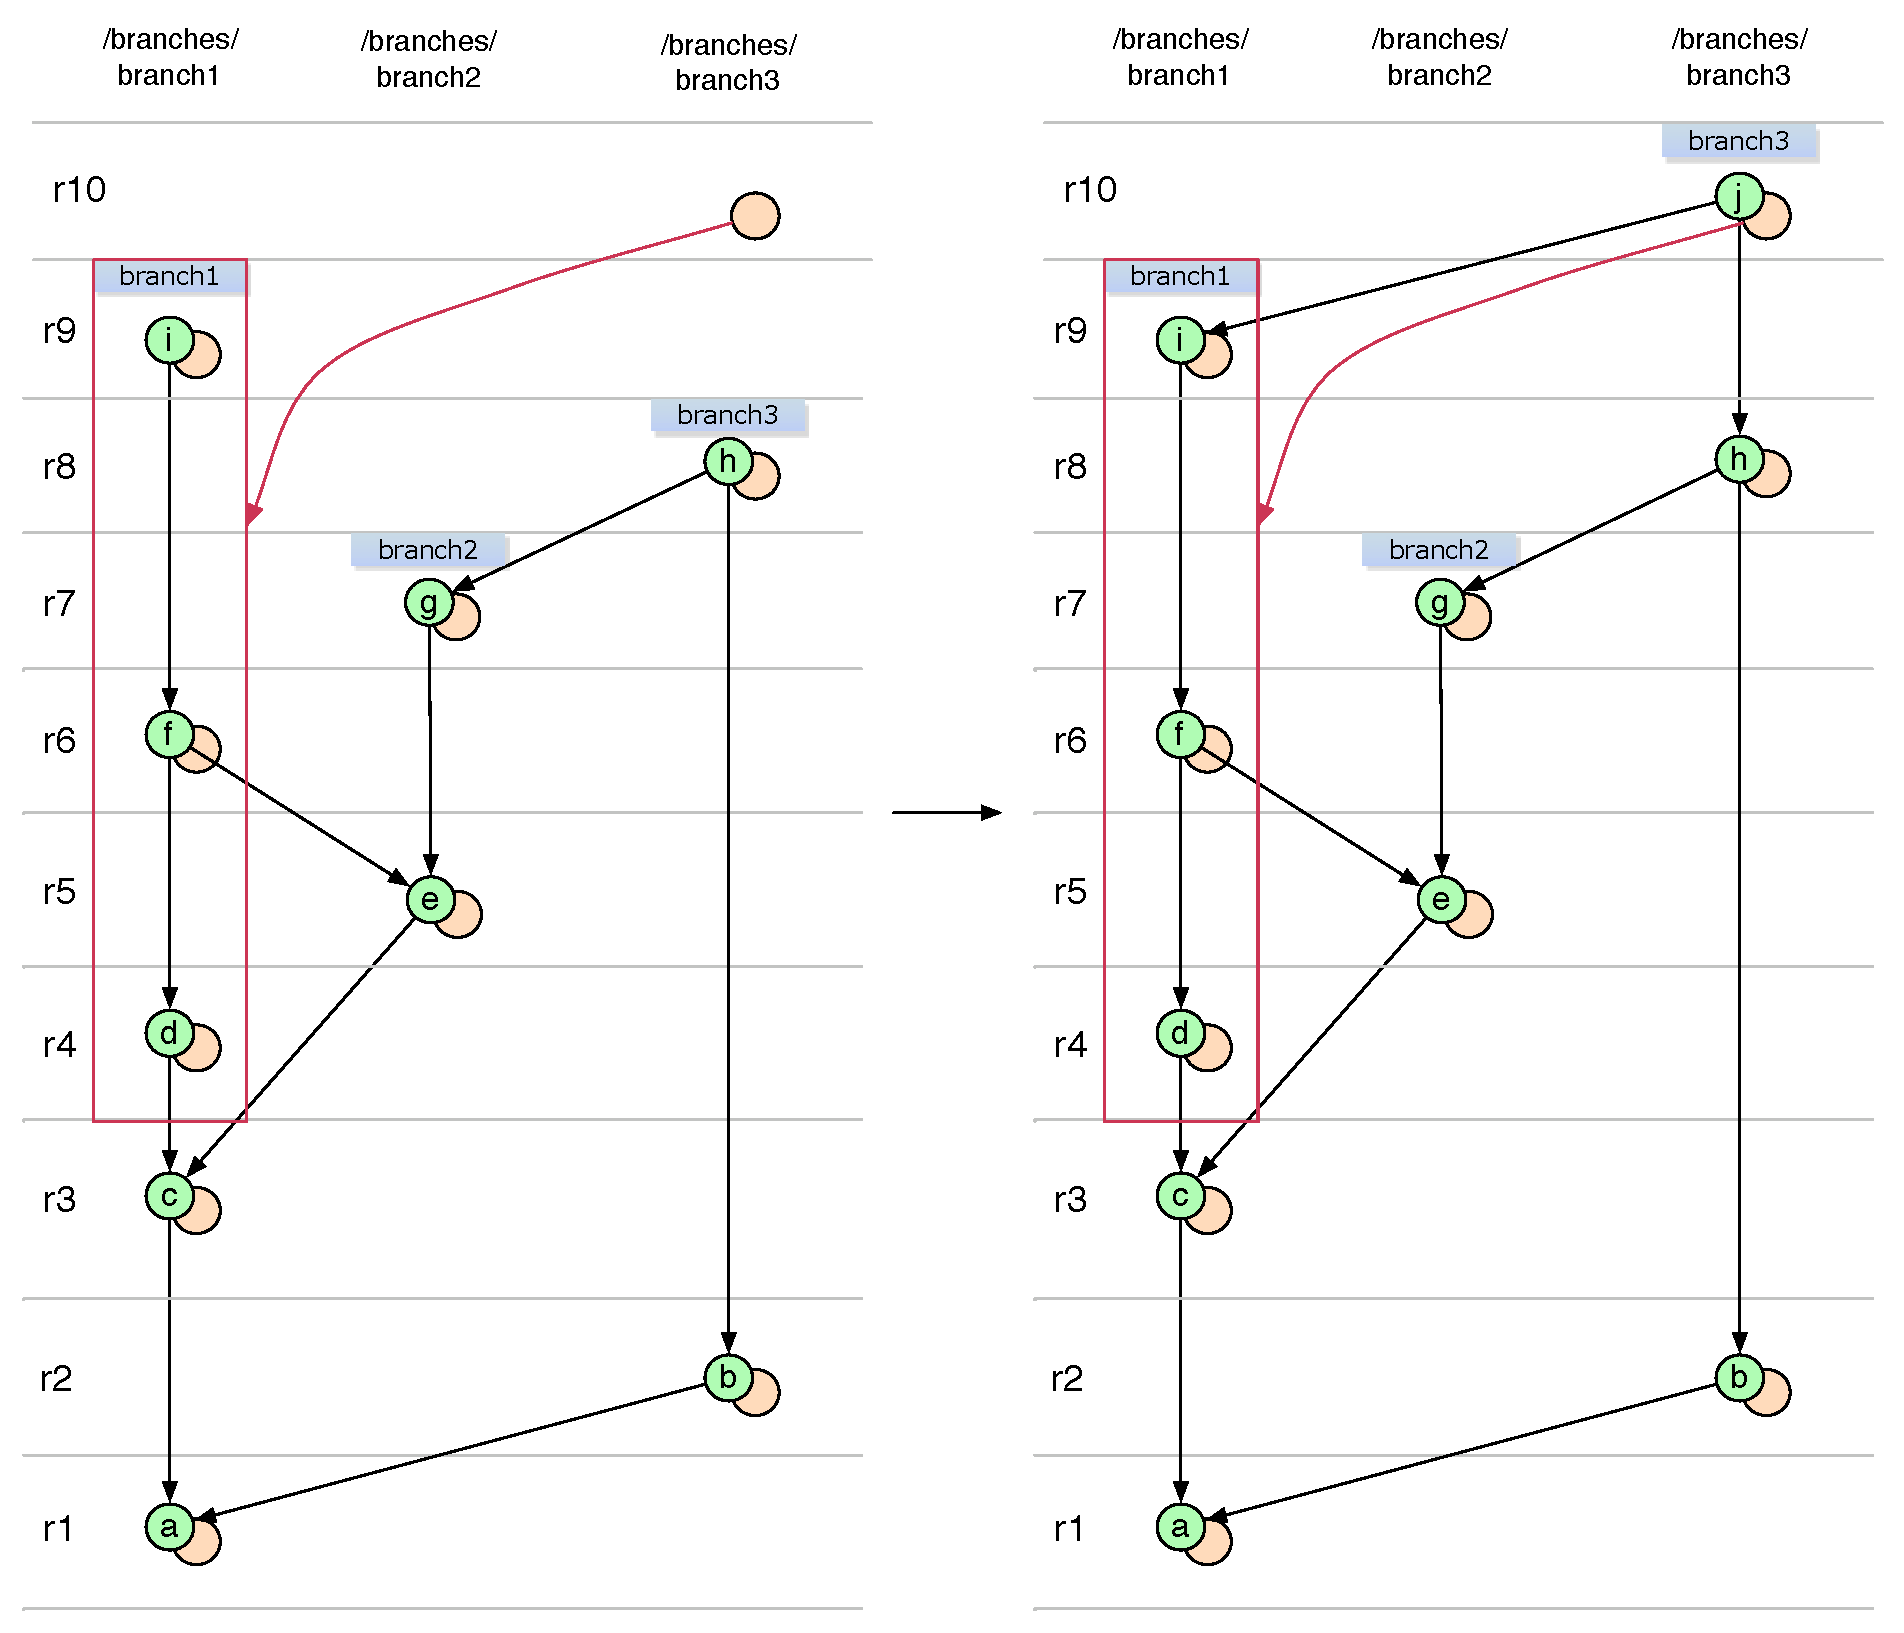
\includegraphics[width=\textwidth]{img/diagrams/merge_sequence_svn_to_git.pdf}%
\captionof{figure}{Merge of Git branch which is available from another branch being translated to a sequence of Subversion revisions.}
\label{merge_sequence_svn_to_git}%
\end{center}

\begin{center}
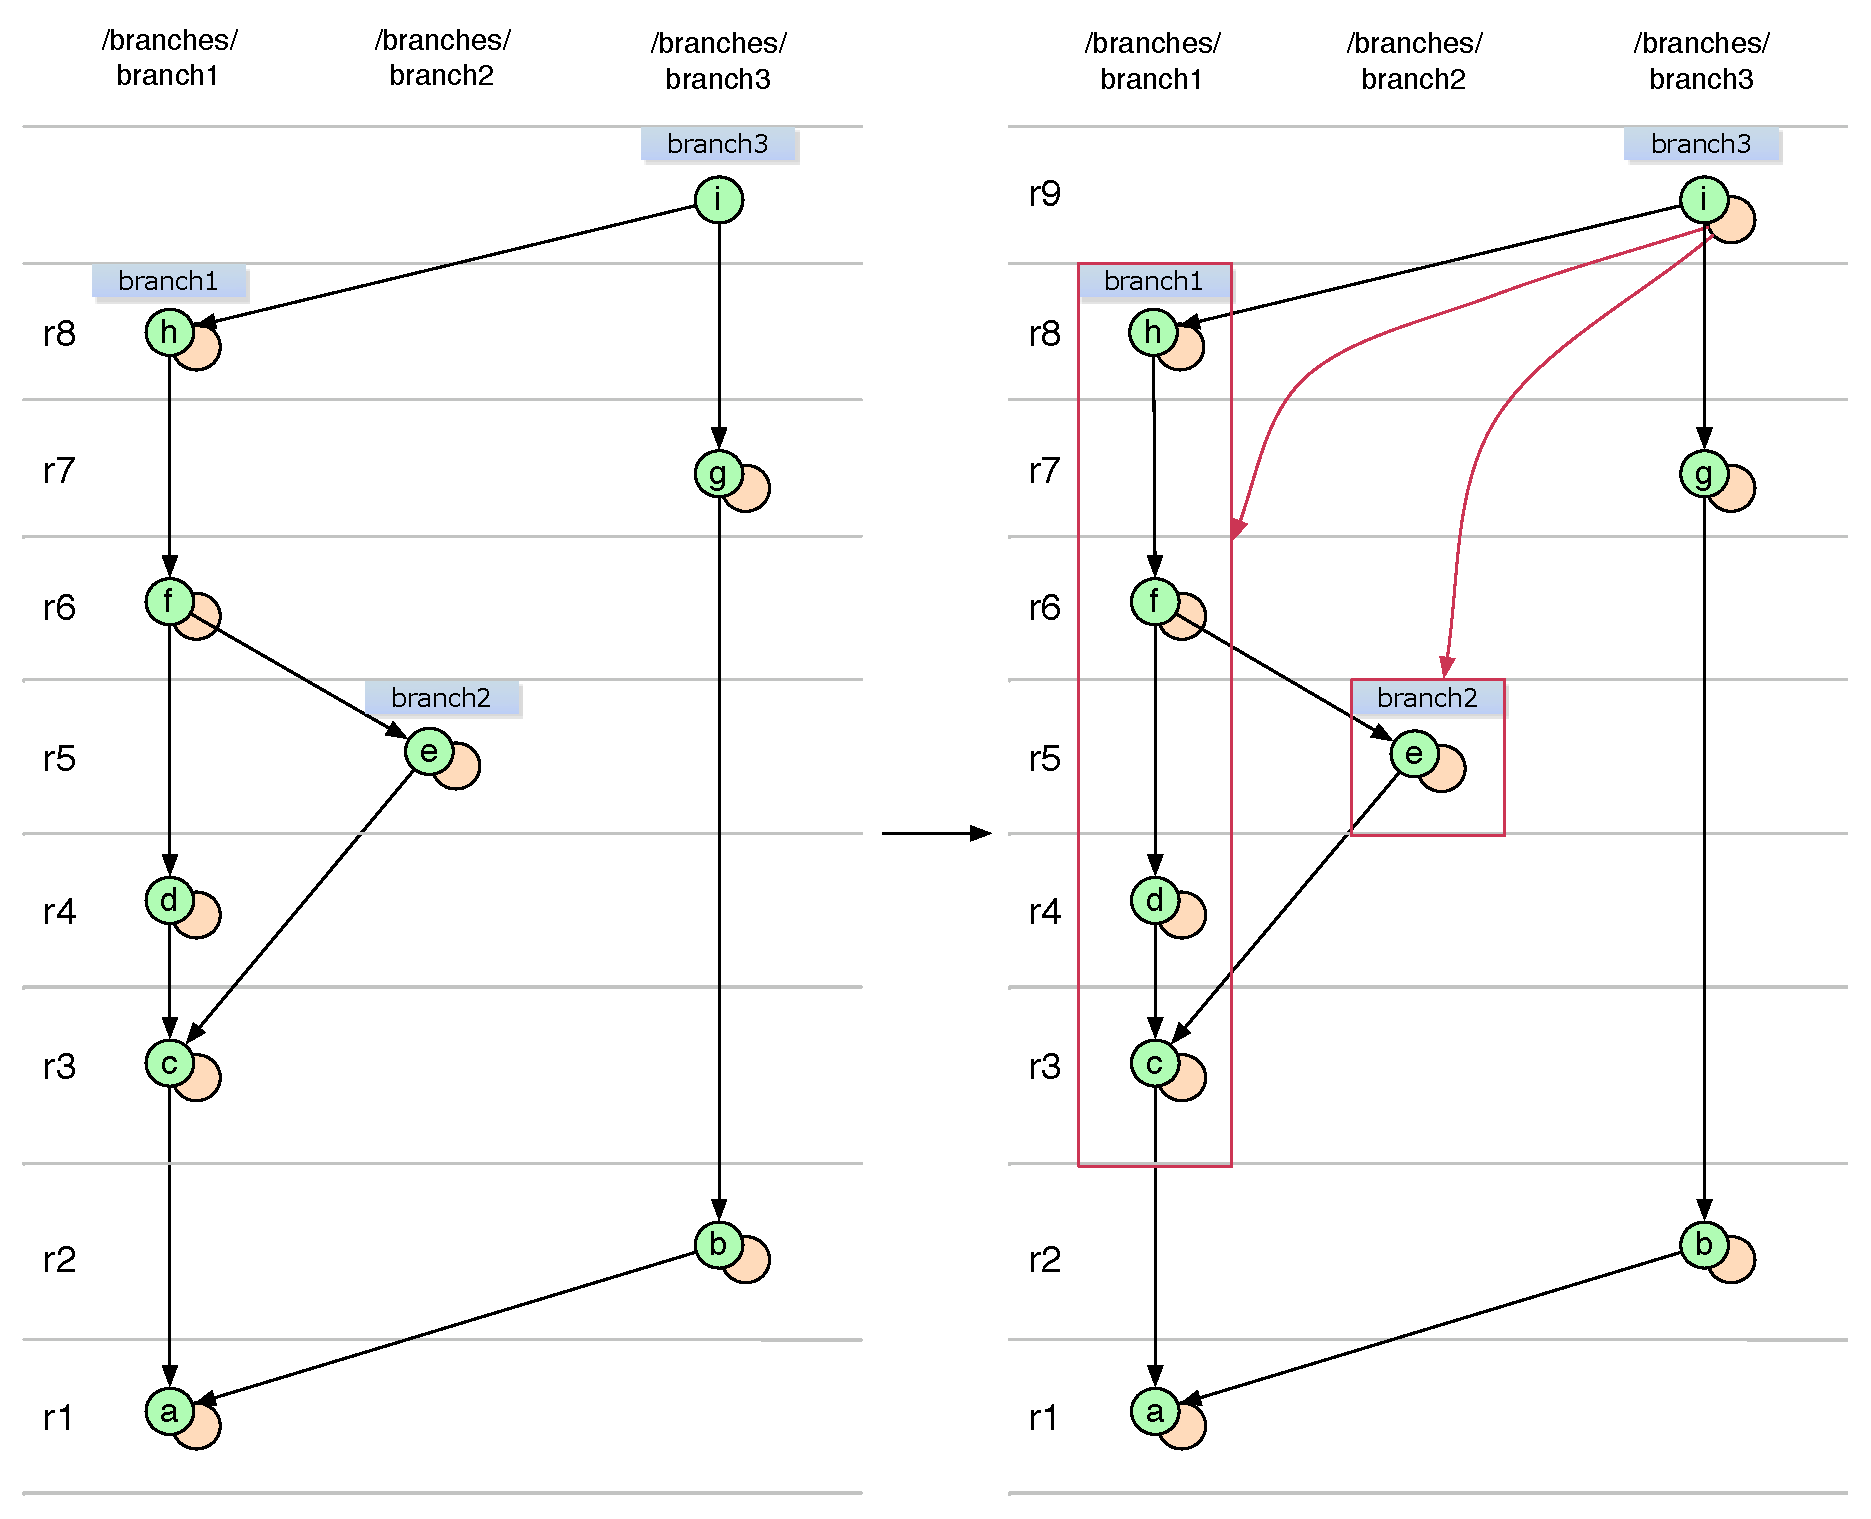
\includegraphics[width=\textwidth]{img/diagrams/nested_merge_full_mergeinfo_git_to_svn.pdf}%
\captionof{figure}{Merge of Git branch which is available from another branch being translated to a sequence of Subversion revisions.}
\label{nested_merge_full_mergeinfo_git_to_svn}%
\end{center}

\begin{center}
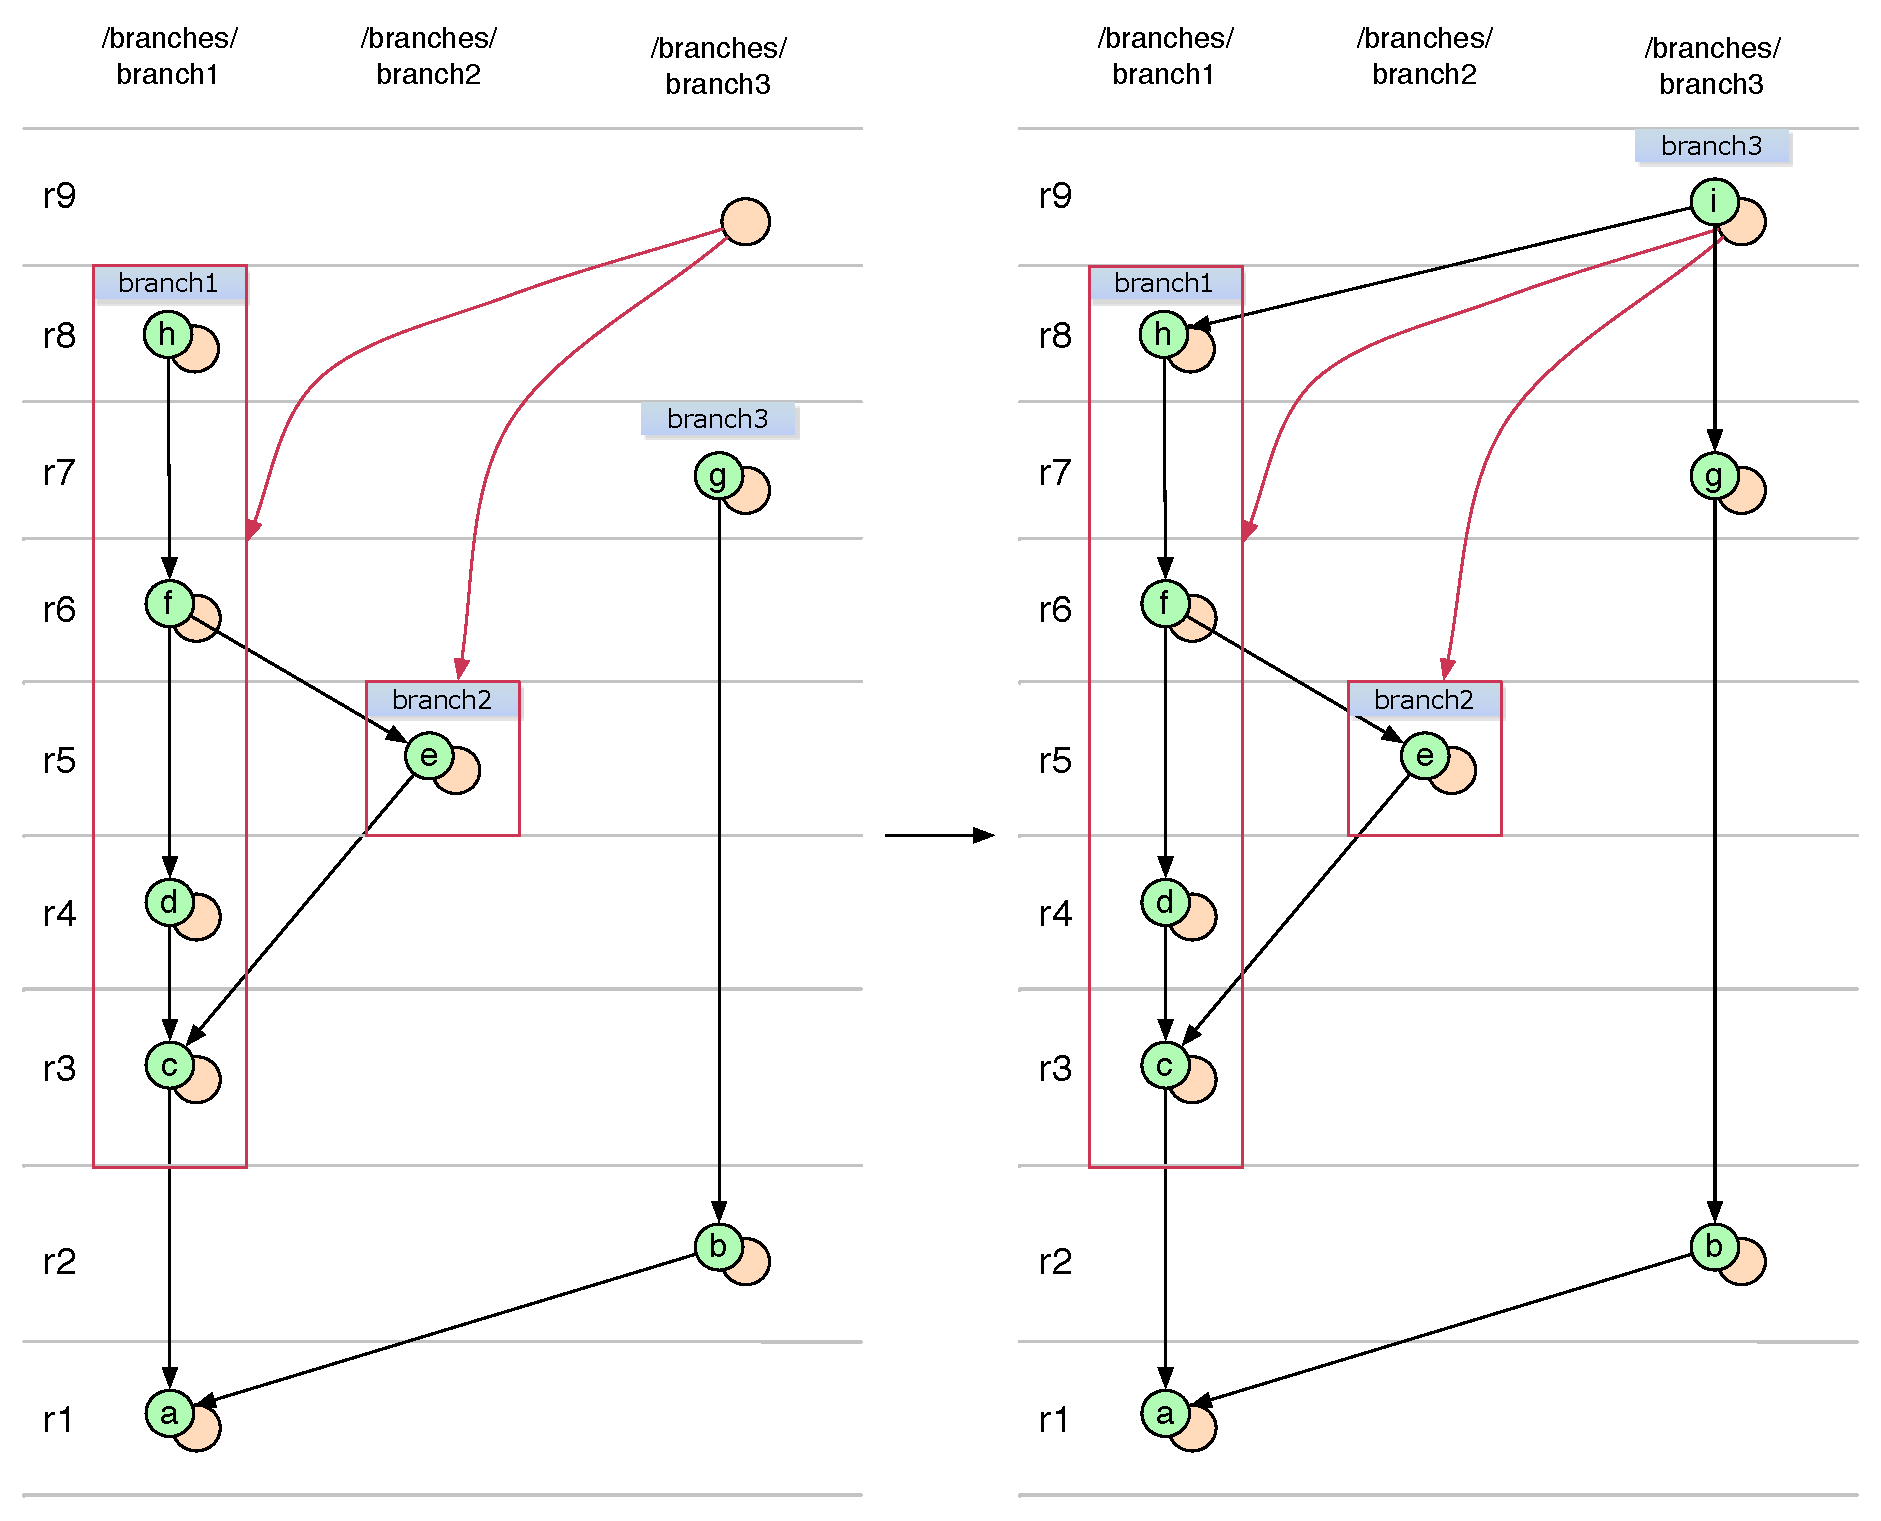
\includegraphics[width=\textwidth]{img/diagrams/nested_merge_full_mergeinfo_svn_to_git.pdf}%
\captionof{figure}{Merge of Git branch which is available from another branch being translated to a sequence of Subversion revisions.}
\label{nested_merge_full_mergeinfo_svn_to_git}%
\end{center}

\begin{center}
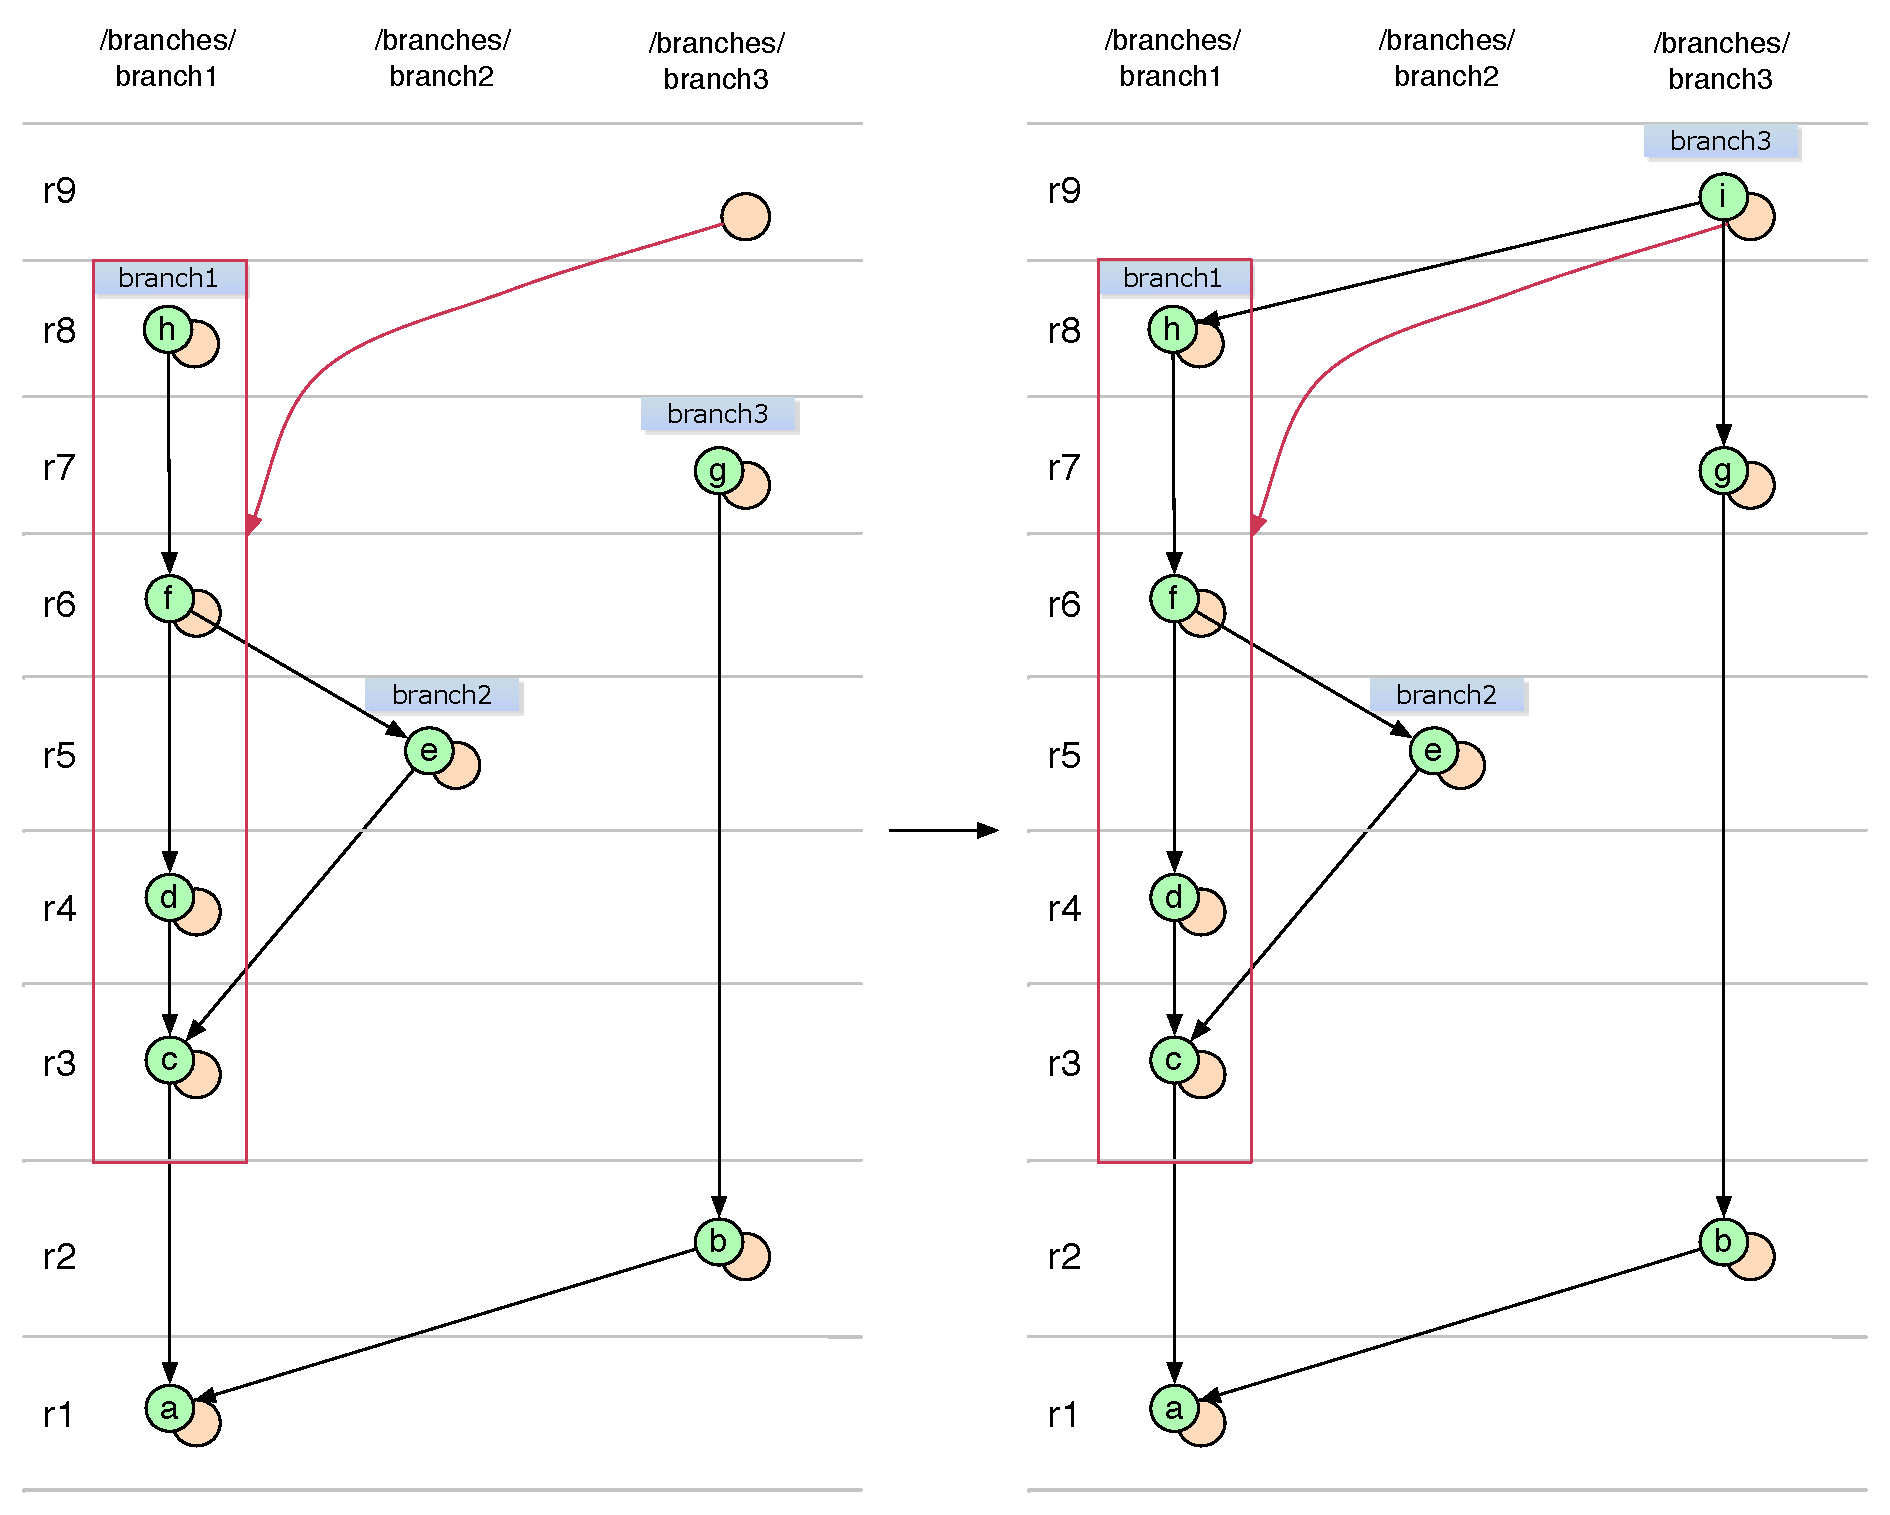
\includegraphics[width=\textwidth]{img/diagrams/nested_merge_partly_mergeinfo_svn_to_git.pdf}%
\captionof{figure}{Merge of Git branch which is available from another branch being translated to a sequence of Subversion revisions.}
\label{nested_merge_partly_mergeinfo_svn_to_git}%
\end{center}

\begin{center}
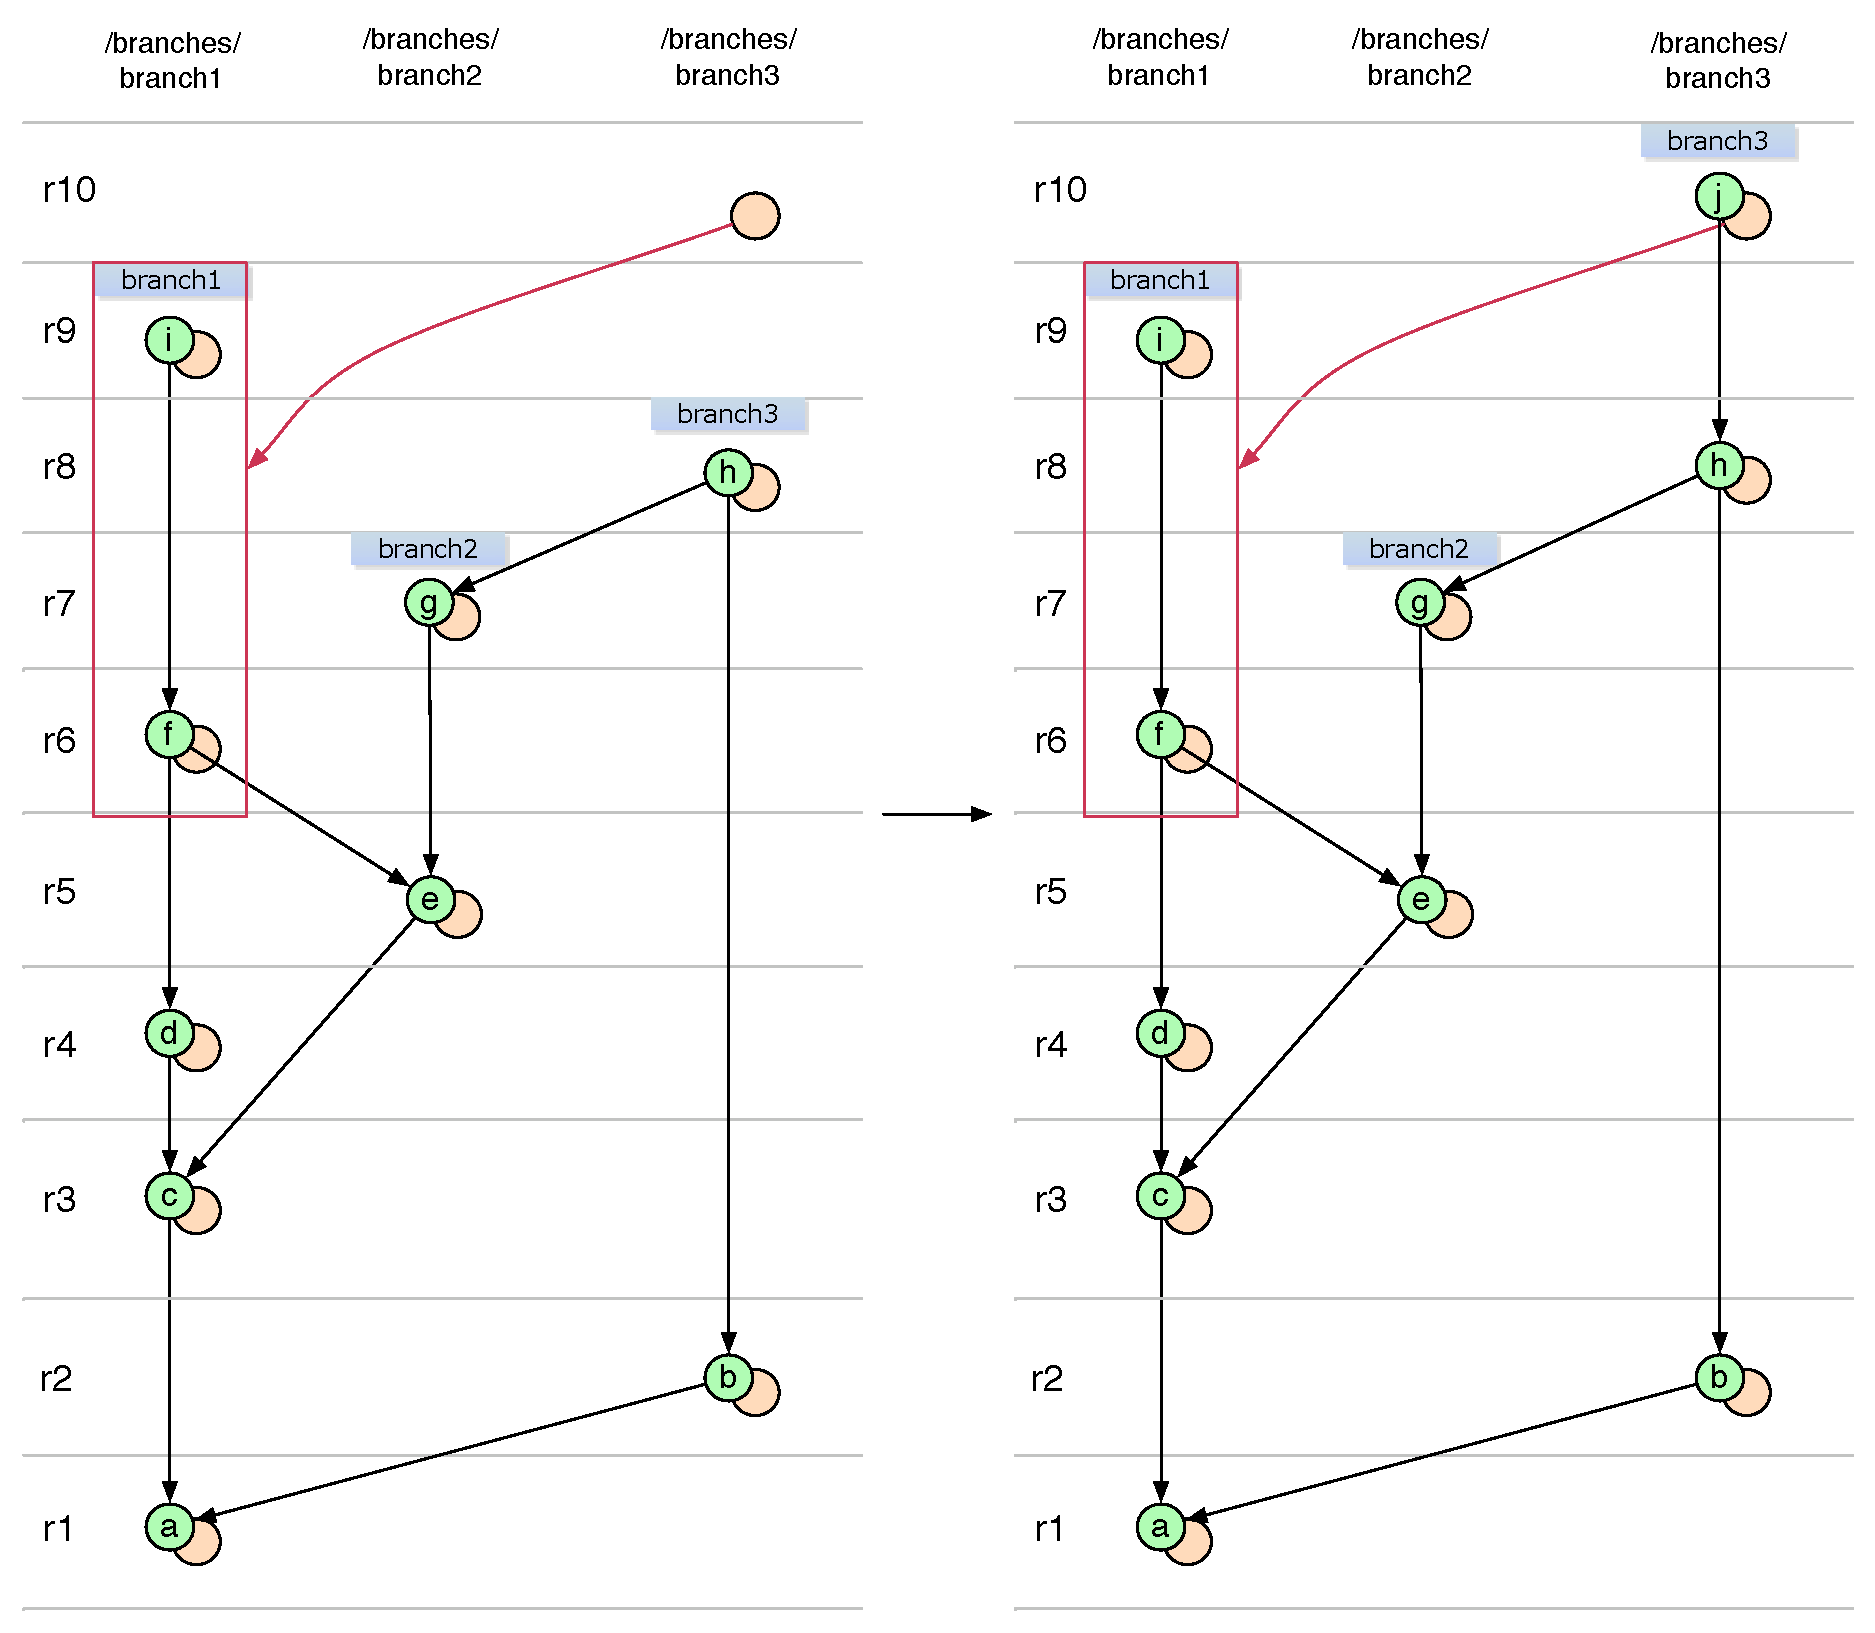
\includegraphics[width=\textwidth]{img/diagrams/no_merge_commit_cherry_pick_sequence_svn_to_git.pdf}%
\captionof{figure}{Merge of Git branch which is available from another branch being translated to a sequence of Subversion revisions.}
\label{no_merge_commit_cherry_pick_sequence_svn_to_git}%
\end{center}

\subsubsection{Octopus Merge}

\begin{center}
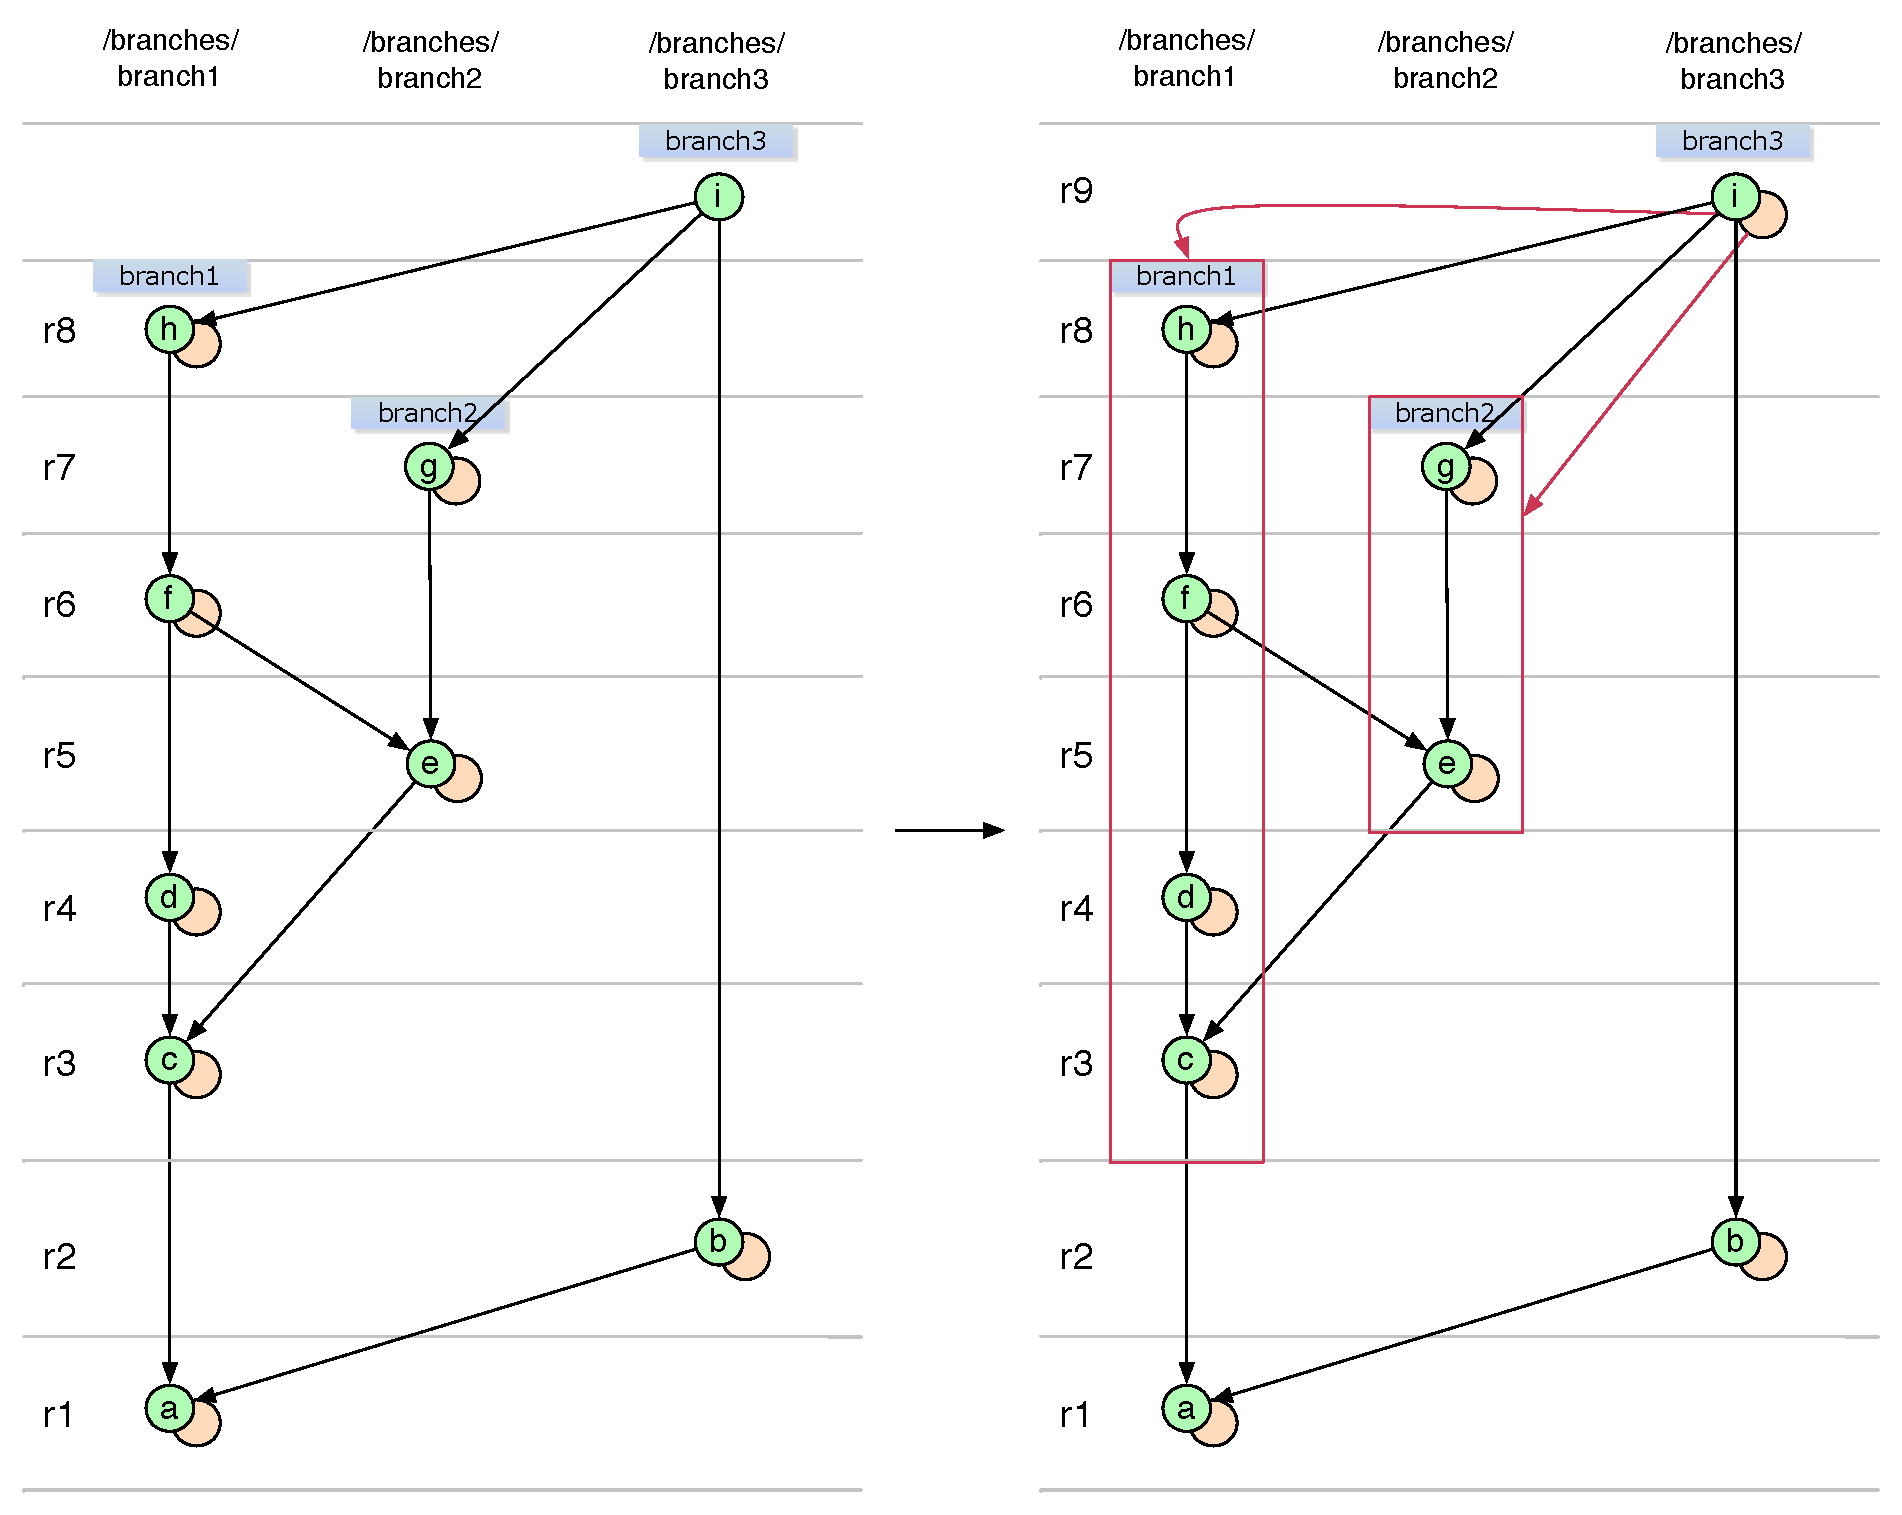
\includegraphics[width=\textwidth]{img/diagrams/octopus_merge_git_to_svn.pdf}%
\captionof{figure}{Octopus merge commit being translated to svn:mergeinfo change.}
\label{octopus_merge_git_to_svn}%
\end{center}

\begin{center}
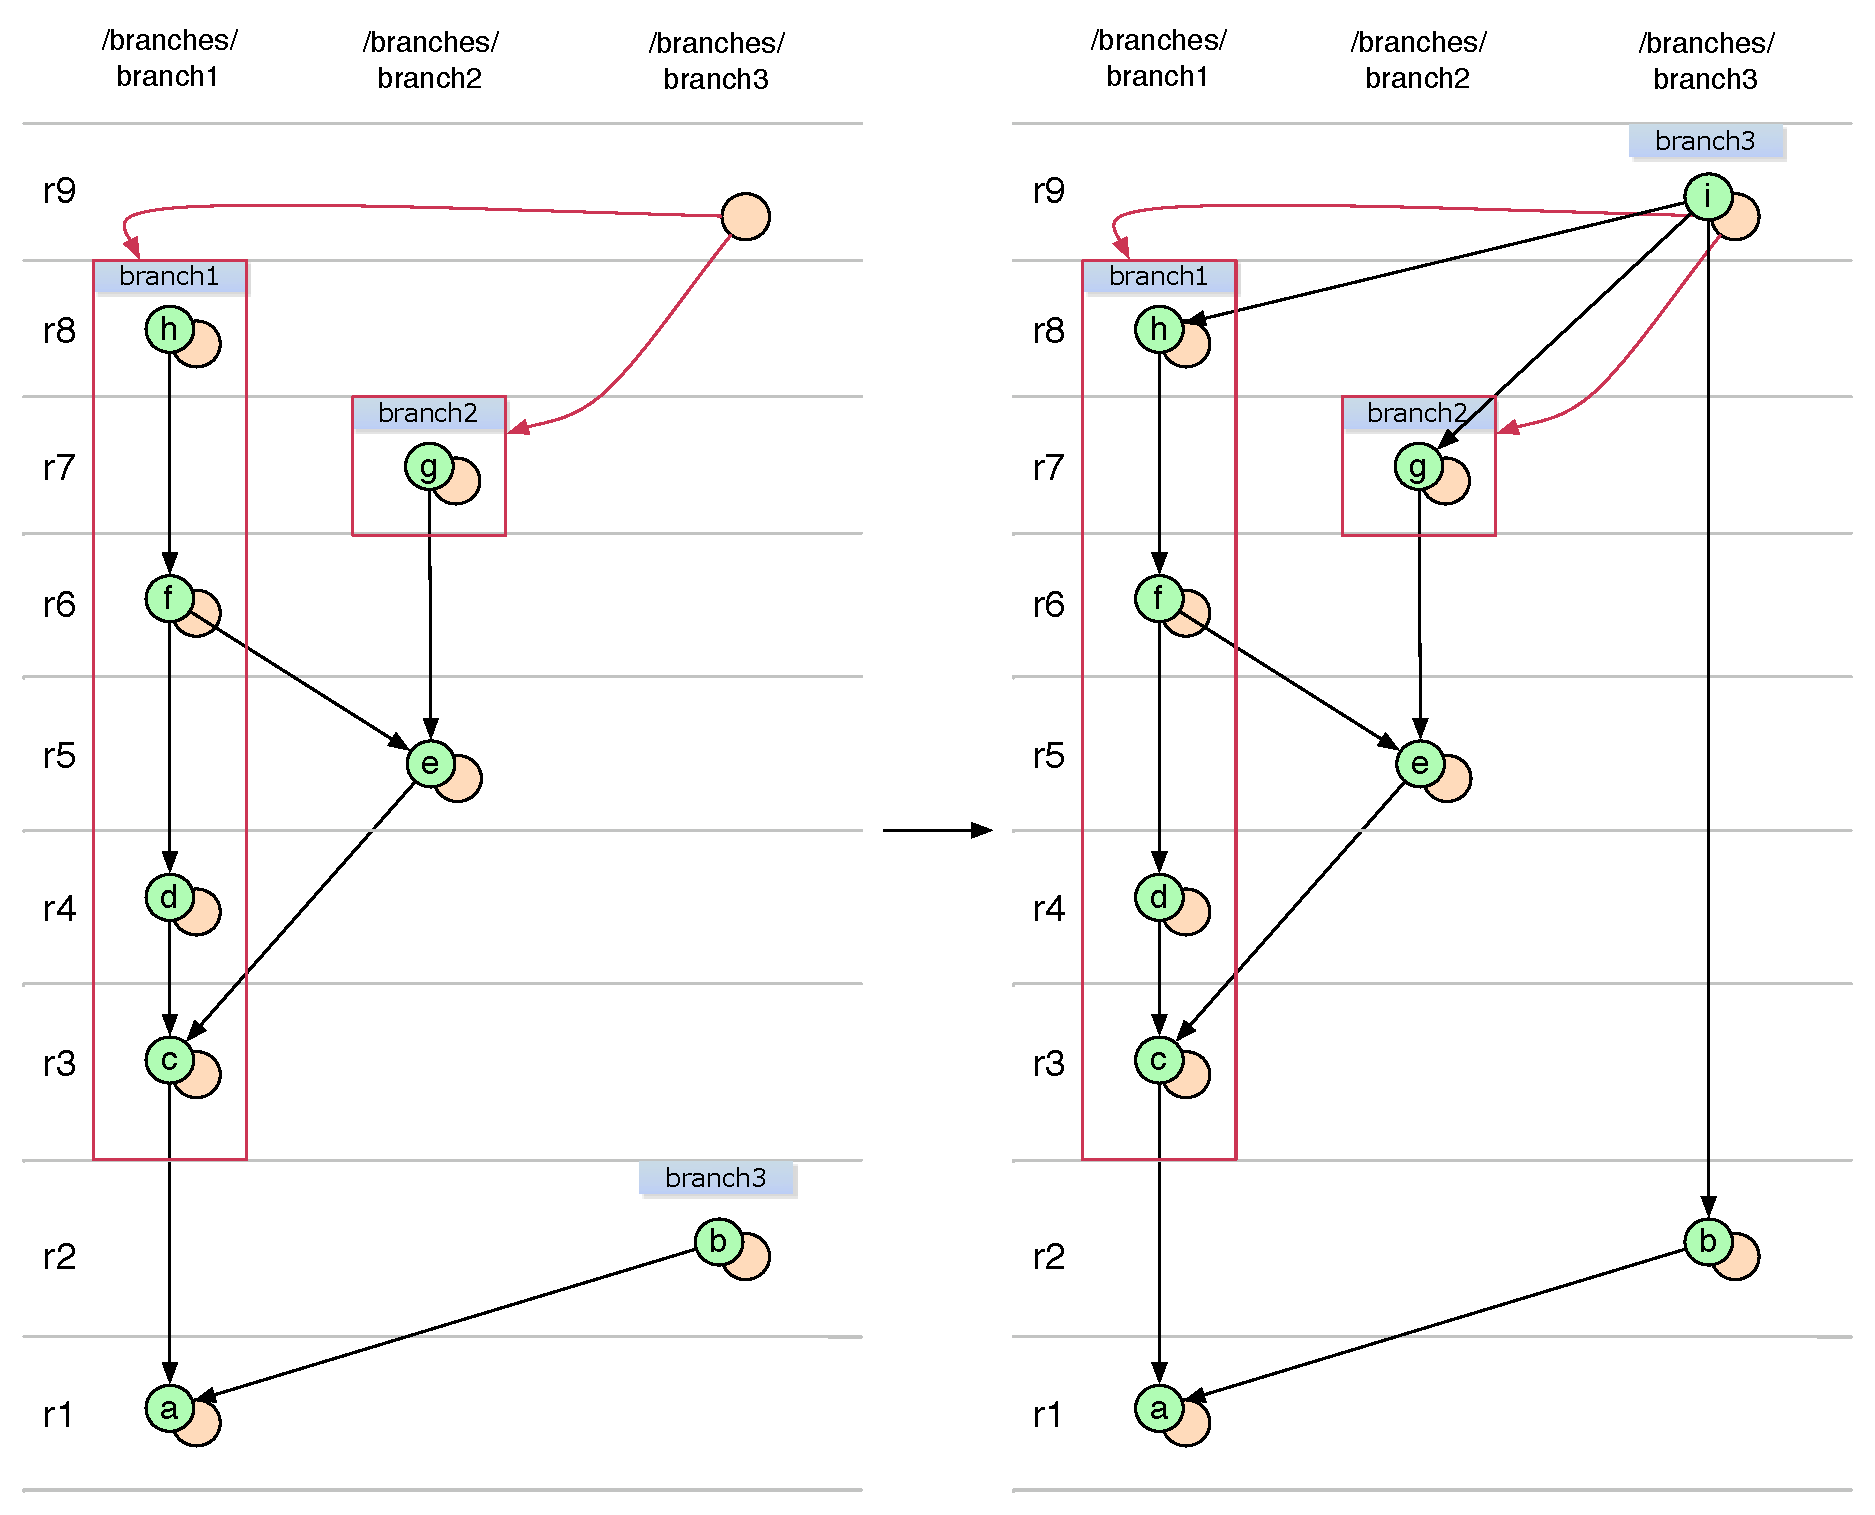
\includegraphics[width=\textwidth]{img/diagrams/octopus_merge_svn_to_git.pdf}%
\captionof{figure}{Change of svn:mergeinfo property being translated to octopus merge commit.}
\label{octopus_merge_svn_to_git}%
\end{center}
